% supplementary.tex -- Supplementary material for the JSS submission
% "Software-as-a-Graph: Heterogeneous Graph Learning for Pre-Deployment
%  Dependability Analysis of Complex Distributed Systems"
%
% Contains the parameter-sensitivity analyses supporting RQ3. Every figure here
% is regenerable from the committed artifacts named in the replication package;
% the main text cites this document rather than reproducing the sweeps.

\documentclass[preprint,3p]{elsarticle}
\usepackage[T1]{fontenc}
\usepackage{lmodern}
\usepackage{amsmath,amssymb}
\usepackage{graphicx}
\usepackage{booktabs}
\usepackage{multirow}
\usepackage{hyperref}
\usepackage{microtype}

\renewcommand{\thesection}{S\arabic{section}}
\renewcommand{\thetable}{S\arabic{table}}
\renewcommand{\thefigure}{S\arabic{figure}}

\journal{Journal of Systems and Software}

\begin{document}

\begin{frontmatter}
\title{Supplementary Material --- Software-as-a-Graph: Parameter Sensitivity of the Explanation Layer}
\author[itu]{Ibrahim Onuralp Yigit}
\author[itu]{Feza Buzluca}
\affiliation[itu]{organization={Department of Computer Engineering, Istanbul Technical University},
             city={Istanbul}, postcode={34469}, country={Turkey}}
\end{frontmatter}

\section{Parameter Sensitivity of the Explanation Layer}
\label{supp:params}

\subsection{Heterogeneous Graph Transformer Message-Passing Formulation}
\label{supp:hgt}

For completeness, we record the layer-wise equations of the Heterogeneous Graph Transformer (HGT) \cite{hu2020hgt} implemented via PyTorch Geometric's \texttt{HGTConv} \cite{fey2019fast} and summarized in Section~4.1.2 of the main manuscript. For source node $u$ and target node $v$ connected by meta-relation $\tau(e) = (\tau(u), \phi(e), \tau(v))$:
\begin{enumerate}
    \item \textbf{Type-Specific Projection:} Raw node features $x_v$ (dimension 19--25) are mapped into hidden dimension $D$:
    \begin{equation}
    h_v^{(0)} = \text{LayerNorm}\big(\text{GELU}(W_{\tau(v)} x_v)\big)
    \end{equation}
    \item \textbf{Relational Mutual Attention:} For attention head $i \in \{1, \dots, H\}$, with incoming neighborhood $\mathcal{N}(v)$ and incorporated edge representation $\tilde{h}_v = h_v + e_{uv}'$:
    \begin{equation}
    \text{Attn}^{\,i}(u, e, v) = \underset{u \in \mathcal{N}(v)}{\text{Softmax}}\left( K^i(u)\, W^i_{\text{att},\phi(e)}\, Q^i(\tilde{h}_v)^\top \cdot \frac{\mu_{\langle \tau(u), \phi(e), \tau(v)\rangle}}{\sqrt{D/H}} \right)
    \end{equation}
    where $\mu_{\langle \tau(u), \phi(e), \tau(v)\rangle}$ is the learned per-meta-relation scaling prior (\texttt{p\_rel} in PyG), weighting entire relation triples independently of individual node embeddings.
    \begin{equation}
    \text{Msg}(u, e, v) = V(u) W_{\text{msg},\phi(e)}
    \end{equation}
    \item \textbf{Residual Aggregation and Layer Normalization:} For layers $l \in \{1, \dots, L\}$:
    \begin{equation}
    h_v^{(l)} = \text{LayerNorm}\left( h_v^{(l-1)} + \text{Dropout}\left(\sum_{u \in \mathcal{N}(v)} \text{Attn}(u, e, v) \cdot \text{Msg}(u, e, v)\right)\right)
    \end{equation}
\end{enumerate}

\begin{table}[htbp]
\centering
\small
\caption{Sensitivity of the RM composite to its ten declared weight constants. \textbf{OFAT} reports one-factor-at-a-time sweeps against $I^*(v)$ over the seven core synthetic domains; \textbf{Morris} reports elementary-effects screening over six scenarios (10 trajectories, 110 evaluations), where $\mu^*$ is influence on mean $\rho$ and $\sigma$ its interaction spread. Rows are ordered by $\mu^*$. Only $r_\alpha$ and $\lambda$ are load-bearing.}
\label{tab:S1}
\resizebox{\linewidth}{!}{%
\begin{tabular}{llcc}
\toprule
\textbf{Constant} & \textbf{One-factor sweep (OFAT)} & \textbf{Morris $\mu^*$} & \textbf{Morris $\sigma$} \\
\midrule
$r_\alpha$ (Fault Tolerance / Availability blend) & not swept individually & $\mathbf{0.132}$ & $0.040$ \\
$\lambda$ (AHP shrinkage, uniform $\to$ raw) & $\rho = 0.319 \to 0.200$, monotone (spread $0.119$) & $\mathbf{0.134}$ & $0.090$ \\
\midrule
$w_{\text{dur}}$ (QoS durability) & \multirow{3}{*}{\parbox{5.2cm}{part of the AHP-derived QoS vector $(0.24, 0.62, 0.14)$; not swept separately}} & $0.013$ & $0.016$ \\
$w_{\text{prio}}$ (QoS priority) & & $0.022$ & $0.024$ \\
$w_{\text{rel}}$ (QoS reliability) & & $0.012$ & $0.018$ \\
\midrule
$\alpha$ (topic payload size) & \multirow{3}{*}{\parbox{5.2cm}{swept jointly over the full $(\beta, \alpha, \psi)$ simplex, 7 points: $w(t)$ ordering never falls below $\rho = 0.919$ against the shipped split; downstream spread $0.031$ (Topo-QoS), $0.007$ (RM)}} & $0.019$ & $0.026$ \\
$\beta$ (topic QoS term) & & $0.025$ & $0.028$ \\
$\psi$ (topic frequency) & & $0.011$ & $0.011$ \\
\midrule
$p$ (power-mean exponent) & not swept individually & $0.005$ & $0.007$ \\
$\gamma$ (library fan-out) & not swept individually & $0.001$ & $0.001$ \\
\bottomrule
\end{tabular}%
}
\end{table}

\noindent Three things follow. First, the parameter risk of the explanation layer is concentrated in two constants, both internal to the RM composite; the QoS-derived weights on which the framework's architectural story rests are not load-bearing for its output. Second, the topic-weight split $(\beta, \alpha, \psi) = (0.75, 0.15, 0.10)$ is a documented convention rather than a tuned parameter --- no choice within its simplex, including uniform weighting, would meaningfully change any result in this paper. Third, Dirichlet sampling over 100 draws of the whole weight vector confirms that the parameterization is stable as a whole: mean $\rho = 0.200$ (sd $0.010$, 90\% interval $[0.185, 0.218]$), with mean Kendall $\tau = 0.826$ and mean top-20\% Jaccard $0.739$ against the shipped ranking.

\paragraph{The elicited weights are anti-predictive, and we keep them anyway}
The $\lambda$ row deserves separate comment because its direction is unfavorable. Rank correlation falls monotonically as the intra-dimension weights move from a uniform prior toward the raw AHP judgment ($0.319 \to 0.200$, Figure~\ref{fig:S1}): expert elicitation makes the ranking worse, by $0.119$. We retain $\lambda = 0.70$ regardless, and the reasoning should be explicit rather than assumed. RM is an attribution instrument, not a ranking model (Section~6.2 of the main manuscript); its purpose is to say \emph{why} a component is fragile in auditable, standards-referenced terms, and rank correlation against a cascade oracle is not the quantity it is built to maximize. Tuning $\lambda$ toward zero would improve a number we do not claim at the cost of the traceability we do. What this sweep establishes is nonetheless a genuine limitation: we have evidence that the elicited weights produce worse rankings and none that they produce better attributions. Validating the attribution itself --- against practitioner judgment, or against the outcome of applying the repairs it recommends --- is outside this study and is the explanation layer's principal open question (Section~8.4 of the main manuscript).

\begin{figure}[htbp]
\centering
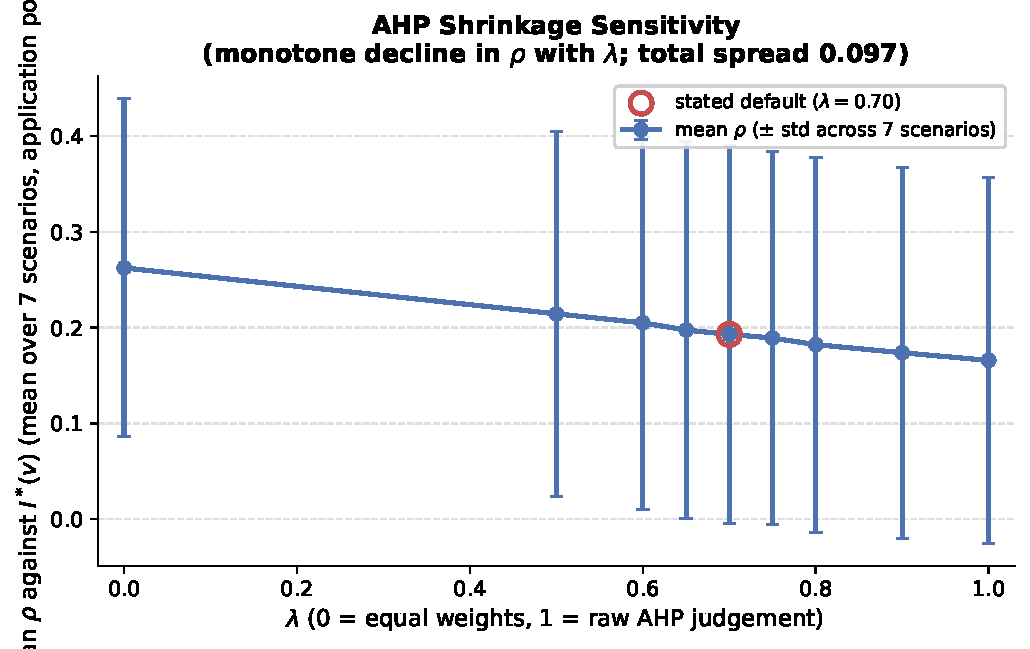
\includegraphics[width=0.62\linewidth]{figures/Figure_S1}
\caption{RM composite rank correlation against $I^*(v)$ across the AHP shrinkage parameter $\lambda$ (Application population, mean over the seven core synthetic domains). The descent is monotone: the closer the intra-dimension weights move to raw elicited judgment, the worse the ranking. Rendered from \texttt{results/ahp\_shrinkage\_sweep\_v3.json}.}
\label{fig:S1}
\end{figure}

\subsection{Global Sensitivity of the Composite Oracle \texorpdfstring{$I_{\text{comp}}$}{I\_comp} Severity Weights}
\label{supp:icomp}

The multi-metric composite failure oracle
\begin{equation}
I_{\text{comp}}(v) = w_1 \cdot \text{ReachabilityLoss} + w_2 \cdot \text{Fragmentation} + w_3 \cdot \text{ThroughputLoss} + w_4 \cdot \text{FlowDisruption}
\end{equation}
defines failure impact across four operational dimensions, parameterized by the AHP-derived severity weights $(0.35, 0.25, 0.25, 0.15)$. Section~7.3.3 of the main manuscript documents that evaluating the RM explanation layer $Q(v)$ against $I_{\text{comp}}(v)$ reveals Simpson's paradox: stratified rank correlations are $\rho = 0.566$ (Application), $0.119$ (Broker), and $0.244$ (Node), while pooling all component types collapses the correlation to $\rho = 0.098$ --- strictly below every per-type stratum it aggregates.

To determine whether this phenomenon is an artifact of the specific AHP weight vector or a structural property of type-heterogeneous aggregation, we conducted two global sensitivity analyses across the 4-simplex ($\sum_{i=1}^4 w_i = 1, w_i \ge 0$) using the manuscript's twelve-scenario corpus (\texttt{results/icomp\_sensitivity\_jss12.json}):
\begin{enumerate}
    \item \textbf{One-Factor-At-A-Time (OFAT) Sweeps:} Each weight $w_i$ is swept across $[0.05, 0.70]$ in 14 increments, proportionally renormalizing the remaining three weights.
    \item \textbf{Uniform Simplex Sampling:} $N = 1{,}000$ weight vectors sampled uniformly on the 4-simplex via $\text{Dirichlet}(1, 1, 1, 1)$, evaluating stratified and pooled Spearman $\rho$ across all scenarios.
    \item \textbf{Morris Elementary-Effects Screening:} Trajectory screening ($r = 15, p = 4$ levels) to isolate the influence of each severity weight on the stratum-separation gap $\Delta = \min(\rho_{\text{app}}, \rho_{\text{broker}}, \rho_{\text{node}}) - \rho_{\text{pooled}}$.
\end{enumerate}

\begin{table}[htbp]
\centering
\small
\caption{Global sensitivity of $I_{\text{comp}}(v)$ severity weights across the 4-simplex ($N = 1{,}000$ Dirichlet draws and Morris elementary-effects screening). Shipped weights: Reachability $0.35$, Fragmentation $0.25$, Throughput $0.25$, Flow Disruption $0.15$. Measured over the manuscript's twelve-scenario corpus. \textbf{Sweep Baseline} is the sweep harness's own evaluation at those weights; it agrees with the canonical detection-benchmark figures quoted in Section~7.3.3 to within $0.002$ on every stratum (see the reconciliation note below).}
\label{tab:S_icomp}
\resizebox{\linewidth}{!}{%
\begin{tabular}{lcccc}
\toprule
\textbf{Stratum / Factor} & \textbf{Sweep Baseline} & \textbf{Dirichlet Simplex Range} & \textbf{Morris $\mu^*_{\text{gap}}$} & \textbf{Morris $\sigma_{\text{gap}}$} \\
\midrule
Application $\rho$ & $0.597$ & $[0.441, 0.599]$ & — & — \\
Broker $\rho$      & $0.317$ & $[0.231, 0.427]$ & — & — \\
Node $\rho$        & $0.140$ & $[0.107, 0.207]$ & — & — \\
Pooled $\rho$      & $0.218$ & $[0.096, 0.351]$ & — & — \\
\midrule
Reachability ($w_1$) & $0.35$ & $[0.05, 0.70]$ & $0.174$ & $0.094$ \\
Fragmentation ($w_2$) & $0.25$ & $[0.05, 0.70]$ & $0.002$ & $0.006$ \\
Throughput ($w_3$) & $0.25$ & $[0.05, 0.70]$ & $0.231$ & $0.075$ \\
Flow Disruption ($w_4$) & $0.15$ & $[0.05, 0.70]$ & $0.143$ & $0.113$ \\
\bottomrule
\end{tabular}%
}
\end{table}

\noindent Table~\ref{tab:S_icomp} establishes three key findings:
\begin{enumerate}
    \item \textbf{Stratum Dominance is Invariant:} Across all $1{,}000$ Dirichlet draws, Application correlation ($\rho \in [0.441, 0.599]$) strictly dominates pooled correlation ($\rho \in [0.096, 0.351]$); the two intervals do not overlap. Heterogeneous pooling degrades ranking performance under 100\% of sampled weight configurations, demonstrating that the failure of pooled evaluations is an intrinsic property of mixing distinct architectural strata rather than an artifact of weight tuning. This is the claim the stratification argument rests on, and it is the one that survives re-scoping: it held on the eight-scenario suite reported previously and holds on the twelve-scenario corpus reported here.
    \item \textbf{The Strict Condition Does Not Hold at the Shipped Weights:} $\rho_{\text{pooled}} < \min(\rho_{\text{app}}, \rho_{\text{broker}}, \rho_{\text{node}})$ holds across $13.9\%$ of the Dirichlet simplex, and the shipped weight vector is not among them: at $(0.35, 0.25, 0.25, 0.15)$ the gap is $-0.078$, because pooled correlation ($0.218$) exceeds the Node stratum ($0.140$). A previous version of this supplement reported the condition as holding at the shipped weights on $34.8\%$ of the simplex; that sweep ran over an eight-scenario suite belonging to a companion study, whose Broker stratum ($\rho = 0.119$ over six scenarios) is far weaker than this corpus's ($0.317$ over eleven). The strict reversal was a property of that suite, not of type-heterogeneous aggregation, and we withdraw it.
    \item \textbf{Dominant Drivers of Separation:} Morris screening demonstrates that Throughput ($\mu^* = 0.231, \sigma = 0.075$) and Reachability ($\mu^* = 0.174, \sigma = 0.094$) are the primary drivers of the stratum gap, with Flow Disruption third ($\mu^* = 0.143$), whereas Fragmentation ($\mu^* = 0.002$) exerts virtually no influence. On the eight-scenario suite Flow Disruption ranked first; the re-ordering is a further consequence of that suite's atypically weak Broker stratum.
\end{enumerate}

\noindent\textbf{Reconciliation with Section~7.3.3.} The \emph{Sweep Baseline} column and the canonical detection-benchmark figures agree, and both are now computed over the same twelve scenarios the rest of the manuscript evaluates. The canonical values come from \texttt{results/detection\_validation\_jss12.json}, produced by running the full \texttt{FailureSimulator}: $\rho = 0.597$ (Application), $0.317$ (Broker), $0.138$ (Node), $0.217$ (pooled); the sweep, which evaluates $I_{\text{comp}}$ as a direct linear combination of four cached per-node severity components and does not re-execute the simulator, reproduces each to within $0.002$. Two corrections are recorded here. First, this note once described a discrepancy of up to $0.035$ between the two procedures and attributed it to that methodological difference; the gap was in fact a defect in the simulator-side evaluation, and correcting it closed the gap on every stratum. Second, and more consequentially, both procedures previously ran over an eight-scenario suite belonging to a companion study, which omits five scenarios of this corpus and includes a regression fixture that appears in no other table of this manuscript. Every figure in this section is now measured over the manuscript's own twelve, and the scenario list is shared by the two scripts rather than duplicated in each.

\section{Zero-Inflation Sensitivity of the Agreement Figures}
\label{supp:zeroinfl}

Spearman $\rho$ over a population where many components are tied at exactly zero is driven substantially by how those ties are handled, and $I^*(v)$ is heavily zero-inflated: $19$ to $106$ Applications per scenario carry exactly zero cascade impact, whereas $I_{\text{comp}}(v)$ has no exact zeros at all. We therefore report, alongside each full-population figure, $\rho_{>0}$ --- the same correlation restricted to components both oracles score strictly positive. It is a sensitivity bound, not a replacement: for a component the simulator actually injected, zero impact is a real measurement ("its failure reaches nobody"), and dropping it would be a results-favorable filter.

The bound changes the reading of two scenarios, in opposite directions. On \texttt{hub\_and\_spoke}, $I_{\text{comp}}$ and $I^*$ correlate at $\rho = -0.044$ over the full population but $\rho_{>0} = +0.263$ over the $22$ components both score positive: the apparent \emph{sign} disagreement is an artifact of tied zeros, not evidence that the oracles order active components inversely. On \texttt{microservices}, the movement runs the other way --- $\rho = 0.461$ falls to $\rho_{>0} = 0.257$, so a substantial part of that scenario's agreement is the two oracles concurring on which components are inert rather than on how the active ones rank. Averaged over the seven scenarios the two summaries are close ($\rho = 0.425$, $\rho_{>0} = 0.447$), which is precisely why the per-scenario figures matter: the mean conceals compensating movements of $0.2$--$0.3$ in both directions.

\section{Domain-Specific Weighting and Threshold Sensitivity}

Sweeping the composite reliability weight $w_R \in [0, 1]$ moves mean $\rho$ by only $0.018$ ($0.317$ at $w_R = 0$ to $0.336$ at $w_R = 1$), and the domain-derived and static rankings agree at mean Kendall $\tau = 0.980$ --- the two orderings are very nearly the same ordering. Within that narrow band the domain-derived weighting does not improve on either alternative it replaces: mean $\rho$ is $0.318$ (domain-derived) against $0.331$ (equal) and $0.321$ (static), so it is marginally the \emph{worst} of the three, losing to equal weighting by $0.013$ and to static by $0.003$. Both margins are far smaller than the between-model differences of Section~7.1 of the main manuscript and we draw no ranking conclusion from either. What the sweep establishes is that no weighting confined to this parameter could move $\rho$ appreciably, so ISO/IEC 25019 context-of-use reweighting must be understood as an attributional device that expresses criticality in stakeholder terms --- and not, on this evidence, as a mechanism that makes the ranking more accurate. Two free parameters of the ground truth itself matter more than any scoring weight, and we sweep both. The cascade propagation threshold moves mean $\rho$ across a spread of $0.084$ ($0.189$ at a threshold of $0$, rising to $0.271$ at $0.5$ and flat thereafter at $0.273$): a permissive threshold that lets every edge propagate produces a noisier target than one that requires meaningful coupling, and the ordering stabilizes once the cutoff reaches $0.5$. Feature normalization spans $0.037$ --- robust scaling at $0.234$ against $0.197$ for both min--max and $z$-score. That is smaller than the threshold spread but of the same order, not negligible beside it: rank-based robust scaling and the two magnitude-preserving alternatives do not induce the same ordering, and the choice is a reported parameter of the scorer rather than an implementation detail. Neither spread indicates that the ordering is \emph{correct}; they indicate only that it is stable under the free parameters of the oracle and the scorer, which is the weaker property a sensitivity sweep can establish.

\section{AHP Pairwise-Comparison Matrices and Their Consistency}
\label{supp:ahp}

Several weight vectors in this framework are derived by the Analytic Hierarchy Process. We state the two that back reported quantities, and we report a property of the matrix family that bears on how much the accompanying consistency ratios are worth.

\paragraph{A caveat on consistency ratios} Saaty's consistency ratio detects \emph{in}consistent judgment; it does not detect a matrix constructed from its own answer. If a priority vector $w$ is chosen first and entry $(i,j)$ is then filled in as $w_i / w_j$, the resulting matrix is perfectly consistent, $CR \approx 0$, and the statistic certifies nothing. Such a matrix is rank-one: every row is a scalar multiple of every other. Writing $\sigma_1 \ge \sigma_2$ for its two largest singular values, the ratio $\sigma_2 / \sigma_1$ separates the two cases --- it is near zero for a back-filled matrix and appreciably positive for one carrying genuine judgment disagreement.

\begin{table}[htbp]
\centering
\small
\caption{Consistency diagnostics for the framework's five AHP matrices. $CR$ alone would suggest all five are sound; $\sigma_2/\sigma_1$ shows that three encode a declared priority vector rather than independent pairwise elicitation. The Availability matrix returns a slightly negative $CR$, which is not attainable for a genuinely elicited matrix ($\lambda_{\max} \ge n$) and arises here as floating-point noise around exact consistency.}
\label{tab:ahp-diag}
\begin{tabular}{lccc}
\toprule
\textbf{Matrix} & \textbf{$n$} & \textbf{$CR$} & \textbf{$\sigma_2/\sigma_1$} \\
\midrule
Topic QoS (main manuscript, Eq.~3) & 3 & $+0.0158$ & $0.072$ \\
Fault Tolerance & 3 & $+0.0029$ & $0.027$ \\
\midrule
Composite impact ($I_{\text{comp}}$) & 4 & $+0.0011$ & $0.014$ \\
Maintainability & 5 & $+0.0005$ & $0.0006$ \\
Availability & 5 & $-0.0029$ & $0.0006$ \\
\bottomrule
\end{tabular}
\end{table}

\noindent Only the Topic QoS matrix carries a consistency ratio that means what a consistency ratio is supposed to mean, and it is the one matrix a continuous-integration test guards on both sides: \texttt{tests/test\_ahp\_shrinkage.py} asserts $0.005 < CR < 0.10$, the lower bound existing precisely as a non-degeneracy check. We report the remaining vectors as declared constants with documented structure rather than as elicited judgment, and note that this reading costs the framework little: the global sensitivity analysis (Section~\ref{supp:params}) finds eight of the ten weight constants to have $\mu^* \le 0.023$, so the ranking results in Section~7 of the main manuscript do not rest on these values being optimal.

\begin{table}[htbp]
\centering
\small
\caption{Saaty matrix over the three Topic QoS dimensions backing $\text{QoS}(t)$ in Equation~(3) of the main manuscript. Geometric-mean priority vector $(0.2385, 0.6250, 0.1365)$; $\lambda_{\max} = 3.018$, $CI = 0.0092$, $RI = 0.58$, $CR = 0.0158$. The shipped constants $(0.24, 0.62, 0.14)$ round this within $0.005$.}
\label{tab:ahp-qos}
\begin{tabular}{lccc}
\toprule
 & \textbf{Reliability} & \textbf{Durability} & \textbf{Priority} \\
\midrule
\textbf{Reliability} & $1$ & $1/3$ & $2$ \\
\textbf{Durability} & $3$ & $1$ & $4$ \\
\textbf{Priority} & $1/2$ & $1/4$ & $1$ \\
\bottomrule
\end{tabular}
\end{table}

\begin{table}[htbp]
\centering
\small
\caption{Matrix over the four composite-impact criteria --- reachability loss (RL), fragmentation (FR), throughput loss (TL), flow disruption (FD) --- backing $I_{\text{comp}}(v)$ (Section~4.3 of the main manuscript). Raw priority vector $(0.389, 0.255, 0.255, 0.100)$; after the framework's $\lambda = 0.7$ shrinkage toward a uniform prior, $(0.347, 0.254, 0.254, 0.145)$, which the shipped $(0.35, 0.25, 0.25, 0.15)$ round. Per Table~\ref{tab:ahp-diag} this matrix is rank-one, so it documents the provenance of those constants without independently justifying them.}
\label{tab:ahp-impact}
\begin{tabular}{lcccc}
\toprule
 & \textbf{RL} & \textbf{FR} & \textbf{TL} & \textbf{FD} \\
\midrule
\textbf{RL} & $1$ & $3/2$ & $3/2$ & $4$ \\
\textbf{FR} & $2/3$ & $1$ & $1$ & $5/2$ \\
\textbf{TL} & $2/3$ & $1$ & $1$ & $5/2$ \\
\textbf{FD} & $1/4$ & $2/5$ & $2/5$ & $1$ \\
\bottomrule
\end{tabular}
\end{table}

\begin{table}[htbp]
\centering
\small
\caption{The Reliability--Maintainability (RM) quality decomposition (supporting Section~5 of the main manuscript).}
\label{tab:S3-rm}
\resizebox{\linewidth}{!}{%
\begin{tabular}{lllll}
\toprule
\textbf{Dimension} & \textbf{Sub-Characteristic} & \textbf{Architectural Question} & \textbf{Underlying Graph Metrics} & \textbf{Role / Remediation} \\
\midrule
\textbf{Reliability ($R$)} & \textbf{Fault Tolerance ($FT$)} & How broadly does failure propagate? & Reverse PageRank on $G^\top$, in-degree, cascade depth & Reliability Eng.: add redundancy, circuit breakers \\
& \textbf{Availability ($A$)} & Is this a single point of failure? & Directed articulation score (raw + QoS-weighted), bridge ratio, CDI & DevOps/SRE: replicate host/broker \\
\textbf{Maintainability ($M$)} & \textbf{Modularity/Modifiability} & How complex and coupled is this? & Betweenness, QoS-weighted out-degree, Code Penalty, clustering & Architect: refactor code, decouple \\
\bottomrule
\end{tabular}%
}
\end{table}

\section{Generative Parameters of the Synthetic Corpus}
\label{supp:genparams}

Table~\ref{tab:genparams} records the configuration behind each synthetic scenario of Table~6 in the main manuscript. It is replication detail rather than a result: the corpus shape a reader needs to interpret the evaluation is in Table~6 itself, and every configuration is committed in the replication package.

\begin{table}[htbp]
\centering
\small
\caption{Generative parameters of the twelve synthetic scenarios (eleven evaluation scenarios plus the ATM case study). Seed and fan-out figures are read from the committed configurations; per-entity counts are in Table~6 of the main manuscript. The modal QoS column gives the most common reliability/durability/priority value and the range of topic shares carrying them, computed from the committed topology rather than the config's declared QoS targets, which domain-driven assignment does not always realize (Section~6.1 of the main manuscript).}
\label{tab:genparams}
\resizebox{\linewidth}{!}{%
\begin{tabular}{lrrrl}
\toprule
\textbf{Scenario} & \textbf{Seed} & \textbf{Pub} & \textbf{Sub} & \textbf{Modal QoS (R/D/P)} \\
\midrule
\textbf{Air Traffic Management (ATM)} & 42 & 1.2 & 2.9 & RELIABLE/VOLATILE/HIGH (41--81\%) \\
\textbf{Autonomous Vehicle (AV)} & 1001 & 2.5 & 5.0 & RELIABLE/TRANSIENT\_LOCAL/HIGH (45--80\%) \\
\textbf{Enterprise Pub-Sub} & 7007 & 3.0 & 4.5 & RELIABLE/TRANSIENT\_LOCAL/MEDIUM (29--79\%) \\
\textbf{Financial Trading} & 3003 & 4.0 & 6.0 & RELIABLE/PERSISTENT/HIGH (40--89\%) \\
\textbf{Healthcare Integration} & 4004 & 2.5 & 3.0 & RELIABLE/PERSISTENT/HIGH (40--88\%) \\
\textbf{Enterprise Integration (ESB)} & 5005 & 2.0 & 7.0 & RELIABLE/TRANSIENT\_LOCAL/MEDIUM (33--67\%) \\
\textbf{Industrial SCADA} & 1902 & 1.1 & 1.0 & RELIABLE/TRANSIENT/HIGH (31--80\%) \\
\textbf{IoT Smart City} & 2002 & 2.0 & 1.5 & BEST\_EFFORT/VOLATILE/LOW (56--75\%) \\
\textbf{Logistics Fleet} & 2104 & 1.8 & 1.9 & RELIABLE/TRANSIENT\_LOCAL/MEDIUM (40--76\%) \\
\textbf{Microservices Mesh} & 6006 & 1.5 & 2.0 & RELIABLE/TRANSIENT\_LOCAL/MEDIUM (40--60\%) \\
\textbf{Real-Time Gaming} & 2003 & 2.6 & 2.8 & BEST\_EFFORT/VOLATILE/HIGH (39--71\%) \\
\textbf{Telecom RAN} & 1801 & 2.2 & 1.6 & RELIABLE/VOLATILE/HIGH (36--67\%) \\
\bottomrule
\end{tabular}%
}
\end{table}

\section{Anti-Pattern Detection and Node-Type Stratification}
\label{supp:detection}

Validated against $I_{\text{comp}}(v)$, the rule-based anti-pattern catalog reaches mean precision $0.244$ and recall $0.900$ ($F_1 = 0.384$) --- but it implicates $93.4\%$ of scored components, so that recall is close to what indiscriminate flagging achieves and the precision is near the base rate. The ATM scaling sweep (29 to 444 components, five seeds, seed-invariant) shows the mechanism: Cohen's $\kappa$ ends at $-0.018$ on the 444-component instance, against $+0.035$ at 29 components, with a flag rate of $92.3\%$ at the largest scale. The path is not monotone --- $\kappa$ rises to $+0.086$ at 148 components before collapsing --- so we do not claim a clean decay law, only the endpoint: at the largest scale the catalog's agreement with the oracle is indistinguishable from chance, and marginally on the wrong side of it. The catalog does not become wrong at scale so much as it stops discriminating. We report it as a characterization of the catalog rather than a working triage mechanism, and delegate critical-set identification to the continuous rankers of Sections~7.1--7.2 of the main manuscript. A nineteenth detector, \texttt{DEEP\_PIPELINE}, is excluded for path-combinatorial explosion ($247{,}761$ paths on a 29-component fixture).

\noindent\textbf{Stratification vs. Pooling:} Measured against the composite oracle $I_{\text{comp}}(v)$ over the twelve scenarios of the corpus, stratified RM rank correlations are $\rho = 0.597$ (Application, 12 scenarios), $0.317$ (Broker, 11 scenarios), and $0.138$ (Execution Host, 12 scenarios), while pooled correlation across all types is $\rho = 0.217$. Pooling node types conflates disparate structural base rates across architectural layers, leaving the pooled figure at less than two fifths of the Application stratum. It is not a strict Simpson reversal on this corpus: pooled correlation sits above the Node stratum ($0.138$). This is why every evaluation in this paper is reported on a single stratum, and why pooled critical-set numbers should be read as inflated wherever they appear (Section~7.4 of the main manuscript). On that same pooled benchmark, unweighted degree centrality attains $\rho = 0.314$ and $F_1 = 0.459$ against RM's $0.217$ and $0.350$ --- RM is beaten by degree on both, confirming that it serves as an attribution instrument rather than an unconstrained global ranker.

\section{Explanation Layer on the Open-Source System Models}
\label{supp:rq4}

We evaluated the framework on hand-authored architecture models of five open-source systems (Section~6.1 of the main manuscript), written as dedicated adapters from the systems' public documentation, with results presented in Table~\ref{tab:9supp}. We note the scope of this evaluation before reporting it. Online Boutique is a vendor demonstration application and Train-Ticket an academic benchmark, Home Assistant is an authentic open-source IoT automation platform, and EdgeX Foundry is an industrial edge computing reference implementation; each is an abstraction of its upstream repository rather than a complete transcription; and their labels come from the same simulation oracle used throughout, so what follows tests topological generalization, not agreement with observed field failures. Two further limits bound what this table can support. First, the predictor scored in Table~\ref{tab:9supp} is the deterministic explanation layer $Q(v)$ together with the two training-free topological baselines; the learned model is evaluated separately in Section~7.4.1 of the main manuscript. Both are scored against $I^*(v)$, but under different injector settings (see the caption), so the two tables are not commensurable. Second, the labels are strongly tied at zero in several architectures --- 13 of 32 Applications in Autoware, 14 of 22 in Cloud Microservices, 27 of 41 in Train-Ticket, and 12 of 22 in EdgeX carry zero simulated impact (the complement of the ``Impactful Apps'' column), whereas Home Assistant exhibits much lower zero-inflation with 17 of 24 applications actively participating in failure cascades. Spearman $\rho$ over populations that are heavily tied is dominated by how those ties are handled; the values below use midrank ties throughout.

\begin{table}[htbp]
\centering
\small
\caption{Open-source reference systems scored by the deterministic explanation layer RM / $Q(v)$ --- no GNN checkpoint is invoked, so $\pm$ is oracle variance over five simulation seeds, not training variance. ``Gain vs.\ Deg'' is $\rho_{Q} - \rho_{\text{deg}}$. Ground truth here is $I^*(v)$ (cascade reachability injection) --- the same oracle as Table~12 of the main manuscript, but run with the validation CLI's cascade-depth cap of 5 and averaged over five injector repeats per node, where Table~12's labels run to unlimited depth. Simulator-derived labels, not observed incidents.}
\label{tab:9supp}
\resizebox{\linewidth}{!}{%
\begin{tabular}{lcccccccc}
\toprule
\textbf{System model} & \textbf{$|V|$} & \textbf{$|V_{\text{app}}|$} & \textbf{Spearman $\rho$} & \textbf{Kendall $\tau$} & \textbf{App Overlap@$K$} & \textbf{Pooled Overlap@$K$} & \textbf{Impactful Apps} & \textbf{Gain vs.\ Deg} \\
\midrule
\textbf{Autoware.universe (ROS 2)} & 75 & 32 & \textbf{0.685 $\pm$ 0.010} & 0.513 & 0.333 & 0.800 & 19 / 32 & +0.357 \\
\textbf{Cloud Microservices Mesh} & 60 & 22 & \textbf{0.778 $\pm$ 0.001} & 0.639 & 0.500 & 1.000 & 8 / 22 & +0.014 \\
\textbf{Train-Ticket Booking Mesh} & 90 & 41 & \textbf{0.759 $\pm$ 0.001} & 0.605 & 0.625 & 1.000 & 14 / 41 & +0.264 \\
\textbf{Home Assistant (Smart Home)} & 63 & 24 & \textbf{0.514 $\pm$ 0.016} & 0.373 & 0.250 & 0.667 & 17 / 24 & +0.289 \\
\textbf{EdgeX Foundry (Industrial IoT)} & 63 & 22 & \textbf{0.800 $\pm$ 0.015} & 0.563 & 0.000 & 1.000 & 10 / 22 & +0.427 \\
\bottomrule
\end{tabular}%
}
\end{table}

\noindent\textbf{Key Insights for RQ4:}
\begin{enumerate}
    \item \textbf{The explanation layer ranks unseen architectures well, but this is not a learned-transfer result.} RM / $Q(v)$ attains $\rho = 0.800$ on EdgeX Foundry, $0.778$ on Cloud Microservices, $0.759$ on Train-Ticket, $0.685$ on Autoware.universe, and $0.514$ on Home Assistant. Because $Q(v)$ is a closed-form scoring function rather than a fitted model, applying it to a new architecture involves no transfer in the inductive sense of Section~7.2 of the main manuscript: nothing was trained, and no distribution shift is being survived. What this table establishes is that the deterministic attribution of Section~5 of the main manuscript remains informative on architectures we did not generate. The learned model is a separate question, answered in Section~7.4.1 of the main manuscript.

    Table~\ref{tab:9supp} is not commensurable with Table~8's RM column ($\rho = 0.133$) of the main manuscript, but the cause is not the oracle: Table~8, Table~12 and Table~\ref{tab:9supp} all score against $I^*(v)$ (cascade reachability injection). Table~8 is the synthetic LOSO corpus, whereas Table~\ref{tab:9supp} and Table~12 both score the five system models on the Application stratum; under Table~12's unlimited-depth labels RM attains $\rho = 0.516$ on those same systems. What separates the figures is therefore a real-versus-generated difference together with the injector configuration recorded in the caption, with the tied-label structure described above contributing to both. The practical consequence is that no RM figure in this paper should be compared across tables without checking which population and which injector configuration produced it.

    \item \textbf{Stratified vs.\ Pooled Critical Set Identification:} On the stratified Application population ($V_{\text{app}}$ with $K = \text{round}(0.20 \cdot |V_{\text{app}}|)$), $Q(v)$ identifies the top-20\% critical services with $F_1@K = 0.333$ in Autoware, $0.500$ in Cloud Microservices, $0.625$ in Train-Ticket, $0.250$ in Home Assistant, and $0.000$ in EdgeX Foundry (where failure impact is dispersed broadly across active device services). When evaluated across the pooled multigraph ($K = \text{round}(0.20 \cdot |V|)$), the pooled Overlap@$K$ reaches $0.800$, $1.000$, $1.000$, $0.667$, and $1.000$, respectively. This disparity is the base-rate phenomenon of Section~6.3 of the main manuscript: the passive infrastructure entities (Topics, Nodes, Libraries) carry constant zero failure impact under the injector configuration used for these runs, so a pooled top-$K$ set is largely populated by correctly identifying inert nodes. The pooled column is therefore inflated and we do not read it; the stratified $V_{\text{app}}$ column is the operational figure.
    \item \textbf{Framework Acceptance Gates and Cross-Domain Disparities:} The framework ships a four-condition release gate ($\rho \ge 0.75$, $\text{Overlap@}K \ge 0.70$, $\text{SPOF } F_1 \ge 0.60$, prediction gain $\ge 0.02$). EdgeX Foundry passes all four gates across all five seeds ($100\%$ pass rate), driven by strong rank correlation ($\rho = 0.800$), pooled $F_1 = 1.00$, and robust articulation detection ($\text{SPOF } F_1 = 0.80$). In contrast, the pass rate is zero on the other four architectures: Autoware fails the $\rho$ and SPOF conditions, Cloud Microservices fails SPOF and prediction gain, Train-Ticket fails SPOF, and Home Assistant misses the $\rho$ gate ($\rho = 0.514$) despite scoring a perfect $\text{SPOF } F_1 = 1.00$. What this establishes is a negative result about thresholds, not a positive one about ordering: a gate calibrated on our synthetic corpus fires correctly on one architecture in five, so its absolute cut-offs are domain-specific and do not transfer as shipped. The ordering half of the question --- whether the ranking underneath those thresholds transfers --- is not answered here and is answered negatively in Section~7.4.1 of the main manuscript, once the population is restricted to components that actually propagate a failure.

    \item \textbf{Predictive Advantage over Structural Heuristics:} The ``Gain vs.\ Deg'' column reports $Q(v)$'s rank-correlation margin over an unweighted degree centrality baseline ($+0.427$ on EdgeX Foundry, $+0.357$ on Autoware, $+0.289$ on Home Assistant, $+0.264$ on Train-Ticket, $+0.014$ on Cloud Microservices), so on this population and this oracle the hierarchical attribution of Section~5 of the main manuscript orders components better than degree centrality does. The margin does not generalize beyond those conditions, and we scope it accordingly: on the pooled synthetic detection benchmark of Section~7.3.6 of the main manuscript --- which is measured against $I_{\text{comp}}(v)$ (composite failure simulation) rather than the $I^*(v)$ used here, and across all entity types --- degree \emph{beats} RM on both rank correlation ($0.314$ vs.\ $0.217$) and Overlap@$K$ ($0.459$ vs.\ $0.350$). The two findings are not in conflict --- one is stratified on Applications in five hand-authored system models under $I^*(v)$, the other pooled across types in eight generated ones under $I_{\text{comp}}(v)$ --- but neither supports a general claim that RM dominates degree. Wilcoxon signed-rank tests over the five systems do not reach significance ($p \ge 0.33$), which at $n = 5$ they could hardly do; we report them for completeness rather than as support.

    \item \textbf{The QoS-weighted heuristic was initially unscorable here, and the fix is the substrate.} On the raw multigraph the unweighted \texttt{Topo} reference is computable ($\rho = 0.307 / 0.891 / 0.528$ on Autoware, Online Boutique and Train-Ticket; mean $0.511$) while \texttt{Topo-QoS} is not. The obstacle is not missing QoS data --- every topic in all five adapters carries declared \texttt{durability}, \texttt{reliability} and \texttt{transport\_priority} profiles, and projecting $w(t)$ onto the structural edges yields non-unit weights on $45.3$--$62.2\%$ of them. It is that \texttt{Topo} reads betweenness off the cached \texttt{DEPENDS\_ON} projection, whereas the QoS-weighted variant must recompute it on the raw multigraph, where Applications never route messages and betweenness is identically zero for all of them --- the same degeneracy Section~6.2.1 of the main manuscript gives as the reason topological baselines are run on the projection at all. This is resolved in the reported evaluation: both baselines are scored on the \texttt{DEPENDS\_ON} flow projection, as Section~6.2.1 of the main manuscript prescribes, and Table~12 of the main manuscript therefore carries \texttt{Topo-QoS} on all five systems ($0.289$--$0.888$). Earlier drafts measured the real-world margin against the unweighted reference alone; that gap is closed, and Section~8.4 of the main manuscript records the correction. Separately, projection-based baselines assign constant zero to Applications carrying no derived \texttt{DEPENDS\_ON} edge, accentuating sensitivity to tied ground truth.
\end{enumerate}

\section{HGT Relational Attention Weight Analysis}
\label{supp:attention}

Figure~\ref{fig:S2} visualizes the relational mutual attention distributions of a Heterogeneous Graph Transformer on the ATM case study architecture. \emph{The model is not the predictor evaluated elsewhere in this paper.} It is a three-layer, four-head HGT trained for 100 epochs on the ATM scenario alone at seed 42, built by \texttt{reproduce/extract\_attention.py} for this figure and discarded afterwards. The LOSO-evaluated checkpoints cannot stand in: they are trained over the full corpus, carry a 40-relation schema against this topology's 32, include \texttt{Library} publish and subscribe relations the ATM graph does not contain, and are two layers deep rather than three. Nothing below therefore speaks to what the evaluated predictor attends to; it speaks to whether typed attention differentiates at all.

\begin{figure}[htbp]
\centering
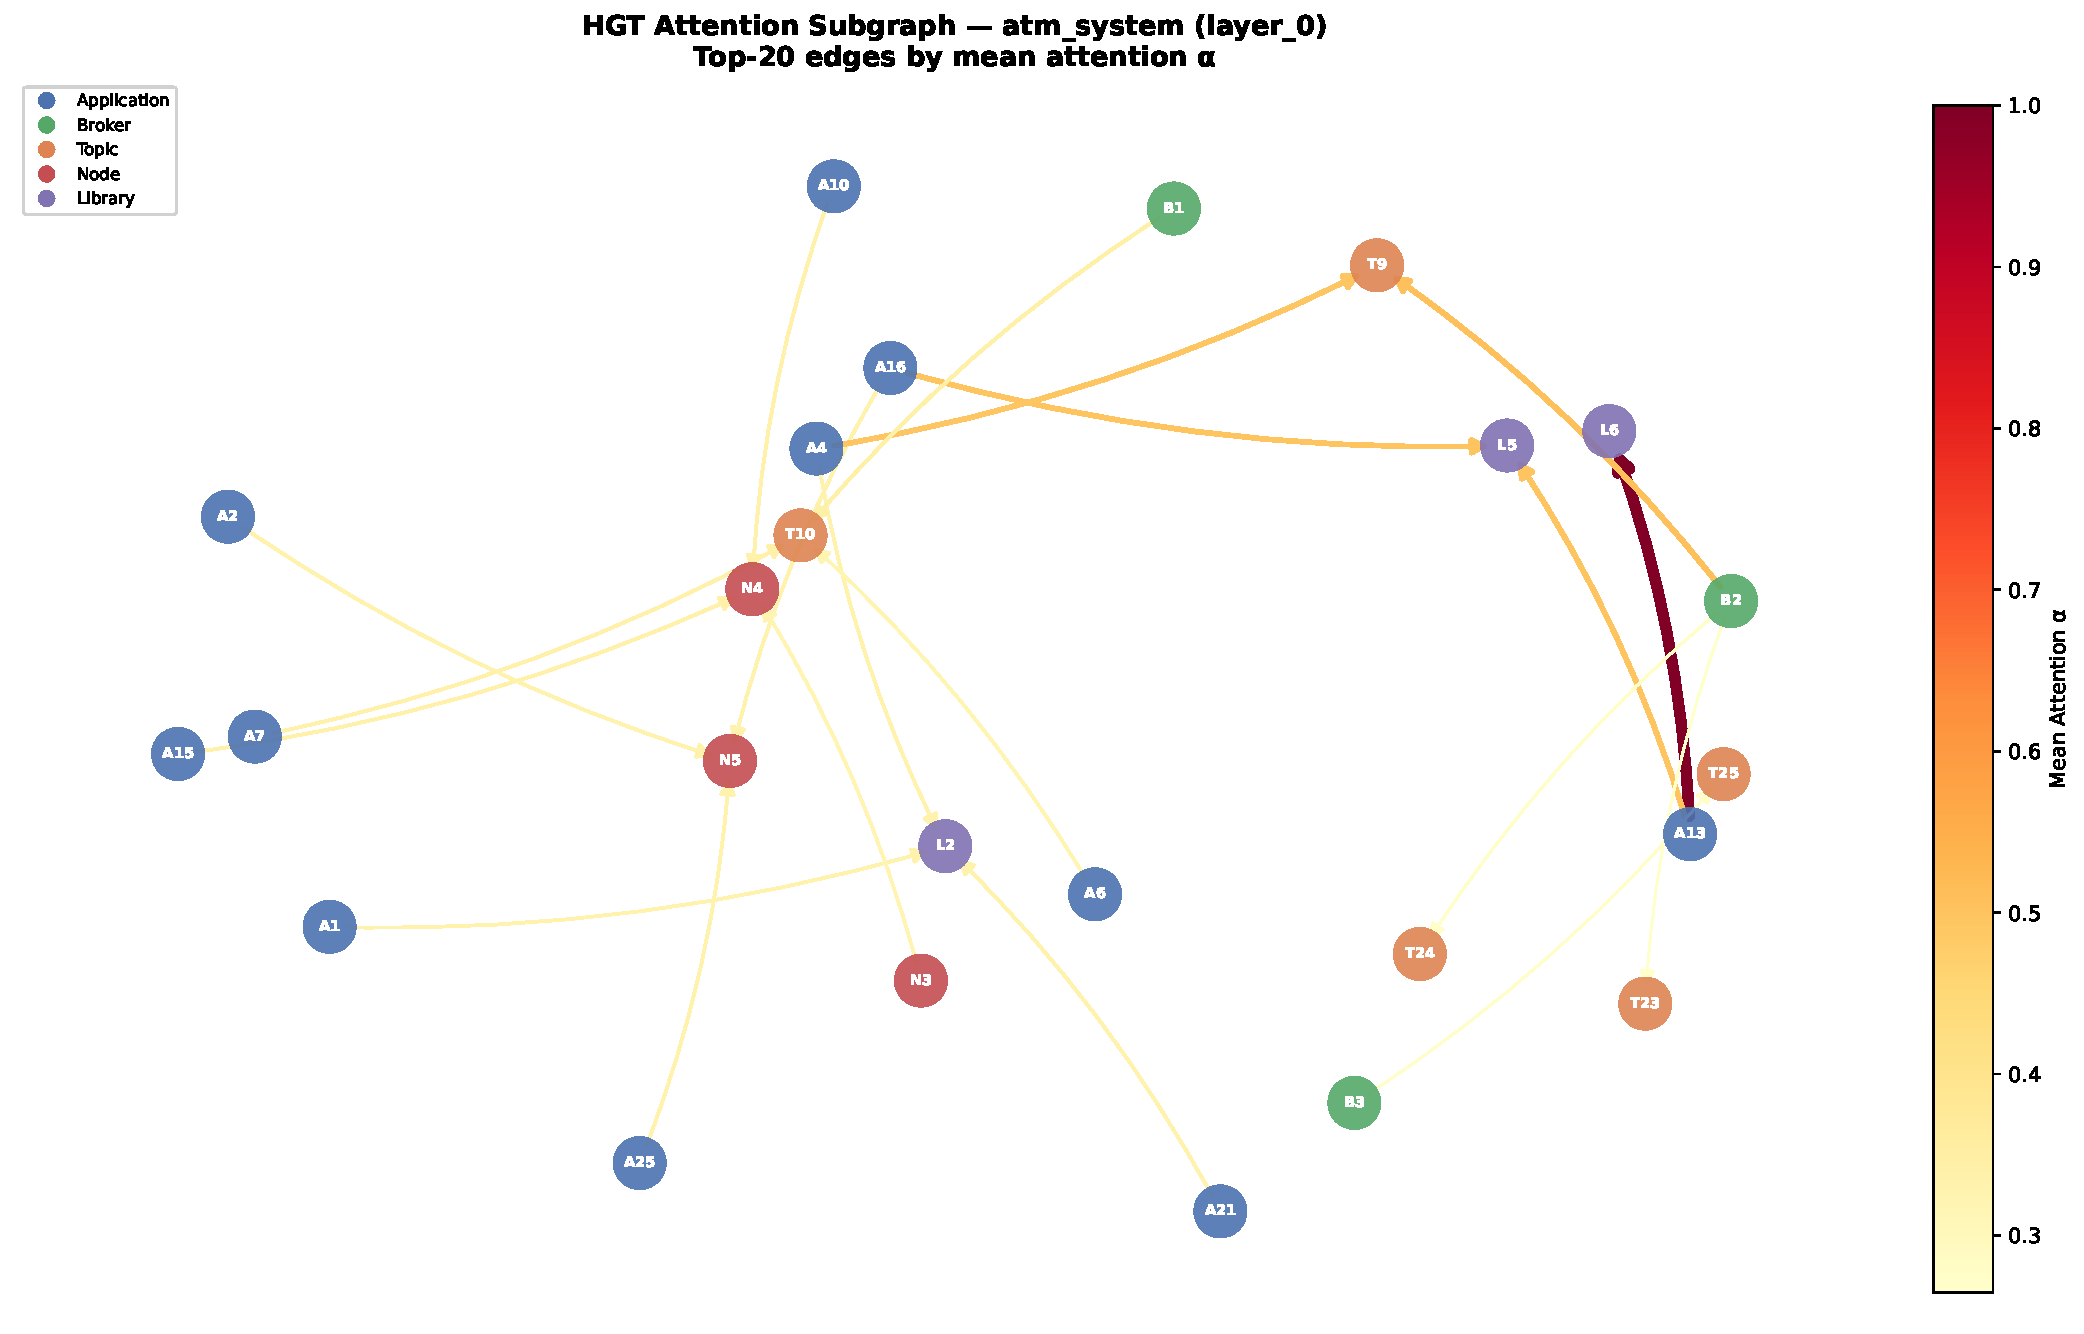
\includegraphics[width=0.75\linewidth]{figures/Figure_S2}
\caption{Relational attention on the ATM case study, from a three-layer HGT trained for 100 epochs on this scenario alone (seed 42) --- not the predictor evaluated in Sections 7.1--7.4 of the main manuscript. Mean $\alpha$ spans $0.113$--$0.222$ across the eight relation types and is governed substantially by destination in-degree. A qualitative illustration on one topology, not evidence of general relation prioritization.}
\label{fig:S2}
\end{figure}

\begin{sloppypar}
Aggregated by relation type, first-layer mean attention across all eight relations runs: \texttt{USES} (App$\to$Lib) $0.220$; \texttt{ROUTES} $0.187$; \texttt{SUBSCRIBES\_TO} $0.172$; \texttt{USES} (Lib$\to$Lib) $0.169$; \texttt{PUBLISHES\_TO} $0.160$; \texttt{RUNS\_ON} (App$\to$Node) $0.156$; \texttt{CONNECTS\_TO} $0.135$; and \texttt{RUNS\_ON} (Broker$\to$Node) $0.113$. Across the three layers no relation-type mean moves by more than $0.019$, but the rank order is \emph{not} stable: the four relations between $0.15$ and $0.18$ are spaced more closely than that drift, and they permute between layers. Three methodological cautions bound what this visualization supports:
\end{sloppypar}
\begin{enumerate}
    \item The spread across all eight relation types is narrow ($0.113$--$0.222$, and only $0.156$--$0.220$ among the five carrying more than nine edges), indicating a mild distributional tendency rather than a clear-cut structural separation.
    \item Because $\alpha$ is computed as a softmax over each destination node's incoming neighborhood $\mathcal{N}(v)$, the mean attention weight $\alpha$ is substantially governed by local in-degree. The single largest weight in the whole extraction ($\alpha_{uv} = 1.00$, on a \texttt{USES} edge into a library) lands on a destination of in-degree one, where $\alpha = 1.0$ holds by arithmetic and carries no information. The thinnest relations sit at the extremes of the ordering: \texttt{USES} (Lib$\to$Lib) carries 3 edges and \texttt{RUNS\_ON} (Broker$\to$Node) carries 5, against 85 for \texttt{SUBSCRIBES\_TO}.
    \item The figure is a function of the corpus snapshot, not a stable property of the architecture. Regenerating the ATM topology changed its edge set without changing any entity count (\texttt{PUBLISHES\_TO} $56 \to 48$, \texttt{SUBSCRIBES\_TO} $90 \to 85$, \texttt{ROUTES} $36 \to 37$, \texttt{CONNECTS\_TO} $7 \to 9$), and that alone moved \texttt{USES} (Lib$\to$Lib) from $0.225$ to $0.169$ --- from above \texttt{ROUTES} to below it. The extraction itself is deterministic, so the whole of that shift is input sensitivity on a 74-node graph.
\end{enumerate}
Consequently, Figure~\ref{fig:S2} serves as an illustrative artifact confirming that multi-head heterogeneous attention remains active across relation types, rather than a statistical proof of general relational importance.

\setlength{\bibsep}{0.5pt}
\bibliographystyle{elsarticle-num}
\bibliography{refs}

\section{Convergent Validity Over Simulation Oracles}
\label{supp:convergent}

We evaluated inter-oracle agreement across $I^*(v)$ (cascade reachability injection), $I_{\text{comp}}(v)$ (composite failure simulation), and $I_{\text{dyn}}(v)$ (dynamic queue-flow simulation) over the twelve inductive folds of Table 5 of the main manuscript, summarized in Table~S3.1:

\begin{table}[htbp]
\centering
\small
\caption{Inter-oracle agreement across simulation paradigms (chance top-$K$ Jaccard is $0.111$) over the twelve LOSO topologies, Application population. One comparison per topology: the five seeds enter $I^*$ only, averaged into a single label per component, while $I_{\text{comp}}$ and $I_{\text{dyn}}$ each run once at seed $42$. $I_{\text{dyn}}$ denotes the queue-flow discrete-event simulation oracle, $I^*$ denotes the graph topological cascade injection oracle, and $I_{\text{comp}}$ denotes the multi-criteria composite oracle. $\rho^{+}$ restricts the correlation to components both oracles score non-zero, separating directional agreement from agreement on which components are harmless. $I_{\text{dyn}}$ was measured under enforced QoS contracts at a calibrated per-subscriber operating point ($\rho_{\text{util}} = 0.65$); the run is reproducible from the commit its artifact names.}
\label{tab:supp-oracles}
\begin{tabular}{lccccc}
\toprule
\textbf{Oracle pair} & \textbf{Mean $\rho$ (range)} & \textbf{Mean $\rho^{+}$} & \textbf{Mean $\tau$} & \textbf{Jaccard@$K$} & \textbf{Tie-robust} \\
\midrule
$I_{\text{dyn}}$ vs.\ $I^*$ & $\mathbf{0.627}$ ($0.186$--$0.953$) & $0.429$ & $0.493$ & $0.370$ & $0.373$ \\
$I_{\text{comp}}$ vs.\ $I^*$ & $0.395$ ($0.083$--$0.653$) & $0.353$ & $0.290$ & $0.266$ & $0.261$ \\
$I_{\text{comp}}$ vs.\ $I_{\text{dyn}}$ & $0.411$ ($-0.073$--$0.705$) & $0.389$ & $0.290$ & $0.324$ & $0.324$ \\
\bottomrule
\end{tabular}
\end{table}

\noindent The queue-flow simulator and the topological cascade oracle agree substantially but not interchangeably ($\rho = 0.627$, Jaccard $0.370$ against $0.111$ expected by chance). \textbf{This is the reading the ceiling supports.} $I^*$'s own seed-to-seed test--retest across these same twelve folds runs $0.811$--$1.000$ (median $0.982$; Section 7.1 of the main manuscript), so $I_{\text{dyn}}$ agrees with $I^*$ distinctly \emph{less} closely than $I^*$ agrees with itself. The gap is the point: a behavioural oracle that reproduced the topological one to within label noise would be re-measuring the topology rather than corroborating it. Ranking over discrete-event queueing traffic recovers most of the topological ordering while retaining content the cascade abstraction does not express.

\noindent Two boundaries qualify this. First, $\rho^{+} = 0.429$ against $\rho = 0.627$ shows that a substantial share of the agreement is the two oracles concurring on which components are \emph{harmless}; restricted to components both score non-zero, agreement is weak in four of twelve folds (Industrial SCADA $-0.069$, Enterprise Integration (ESB) $0.008$, Autonomous Vehicle $0.149$, Microservices $0.194$). Second, Industrial SCADA is the weakest fold ($\rho = 0.186$), and Microservices exhibits the least reproducible label in the corpus (test--retest $0.811$, top-$K$ Jaccard $0.720$), so part of that deficit is label noise rather than construct divergence.

\noindent\textbf{Both oracles have a floor, and only one of them had been measured.} The reading above is stated against $I^*$'s test--retest alone, which silently treats $I_{\text{dyn}}$ as noiseless. It is not: it is a stochastic discrete-event simulation run here at a single seed. Re-running both non-primary oracles across seeds $\{42, 123, 456\}$ on three folds spanning the corpus --- ATM, Healthcare Integration, and Microservices Mesh, the last being the weakest fold above --- gives $I_{\text{comp}}$ a test--retest of $1.000$ everywhere (its Bernoulli cascade draws are effectively deterministic at the shipped edge weights, so its single seed costs nothing), and $I_{\text{dyn}}$ a test--retest of $0.958$--$0.972$ on ATM, $0.828$--$0.867$ on Healthcare, and $0.741$--$0.821$ on Microservices. The subset is three folds rather than twelve because $I_{\text{dyn}}$ costs one discrete-event run per component per seed; it is chosen to bracket the corpus rather than to average over it.

\noindent The consequence is specific. On Microservices, $I_{\text{dyn}}$ agrees with \emph{itself} at $0.741$--$0.821$ --- at or below $I^*$'s own $0.811$ on that same fold --- so the $\rho = 0.337$ reported there is bounded by two dispersions, not one, and attributing the shortfall primarily to $I^*$'s label noise overstates what can be separated. Elsewhere the $0.627$ headline is less affected: on ATM and Healthcare $I_{\text{dyn}}$ reproduces itself at $0.83$--$0.97$, well above the cross-oracle agreement, so the construct-divergence reading of the gap survives on those folds. We report the floors rather than correcting the headline for them, because a noise-corrected correlation would require the twelve-fold multi-seed run this subset stands in for.

\noindent\textbf{Four Golden Signals Telemetry \& Dynamic Contention Relief.} In addition to the scalar delivery rate drop $I_{\text{dyn}}(v)$, each discrete-event execution logs Google SRE's Four Golden Signals (latency, traffic, errors, saturation) windowed across pre-fault ($t < t_{\text{fault}}$) and post-fault ($t > t_{\text{fault}}$) intervals. The queue-level decomposition shows that end-to-end message traversal latency $t_{\text{e2e}}$ is driven by buffer waiting delay under contention ($\rho_{\text{util}} = 0.65$), whereas CPU service processing remains stationary. When a high-throughput publisher fails, surviving subscriber buffers rapidly drain, yielding a pronounced negative correlation between delivery drop $I_{\text{dyn}}$ and tail latency delta ($\rho = -0.499$) as well as deadline violations ($\rho = -0.418$). Preserving the Four Golden Signals as first-class, structured telemetry avoids an additive cancellation trap and equips operators with comprehensive diagnostics alongside the convergent-validity ranking probe.

\section{In-Distribution Significance Tests}
\label{supp:indist}

Paired tests over the twelve in-distribution scenarios of Table 5 of the main manuscript. They are reported here rather than in the body because Section 7.2 declines to read the in-distribution typed--untyped contrast as evidence about typing: the typed pair consumes the native multigraph while the homogeneous pair consumes the Application--Library projection, so the margin mixes typed message passing with multi-entity visibility. The tests are given for completeness, not as support for a claim.

\begin{table}[htbp]
\centering
\small
\caption{Paired Wilcoxon signed-rank tests across in-distribution scenarios ($n = 12$, two-sided).}
\label{tab:supp-indist-wilcoxon}
\resizebox{\linewidth}{!}{%
\begin{tabular}{lrcrcl}
\toprule
\textbf{Comparison} & \textbf{$\Delta\rho$} & \textbf{Won} & \textbf{Wilcoxon $W$} & \textbf{$p$-value} & \textbf{Significance} \\
\midrule
\textbf{HGT-QoS vs. Topo} & \textbf{+0.291} & 11/12 & 2.0 & \textbf{0.0015} & \textbf{Significant} ($p < 0.01$) \\
\textbf{Topo-QoS vs. Topo} & \textbf{+0.198} & 12/12 & 0.0 & \textbf{0.0005} & \textbf{Significant} ($p < 0.001$) \\
\textbf{HGT-QoS vs. GAT-QoS} & \textbf{+0.222} & 11/12 & 3.0 & \textbf{0.0024} & \textbf{Significant} ($p < 0.01$) \\
\midrule
\textbf{HGT-QoS vs. GAT} & $+0.118$ & 9/12 & 21.0 & 0.1763 & Not significant \\
\textbf{HGT-QoS vs. Topo-QoS} & $+0.093$ & 9/12 & 23.0 & 0.2334 & Not significant \\
\textbf{HGT vs. GAT} & $+0.082$ & 8/12 & 29.0 & 0.4697 & Not significant \\
\textbf{HGT-QoS vs. HGT} & $+0.037$ & 8/12 & 32.0 & 0.6221 & Not significant \\
\textbf{GAT-QoS vs. Topo-QoS} & $-0.129$ & 4/12 & 21.0 & 0.1763 & Not significant \\
\bottomrule
\end{tabular}%
}
\end{table}

\section{Typed Node Feature Schema}
\label{supp:features}

Both pathways read the same typed node properties from $G_{\text{analysis}}$: the predictive pathway (Section~4 of the main manuscript) projects them per entity type before heterogeneous message passing, and the explanation layer (Section~5 of the main manuscript) aggregates them into its quality profile. All five entity types share indices 0--17, an 18-dimensional base block of deterministic topological metrics produced by the static analysis stage whose execution cost is characterized in Section~7.6 of the main manuscript. Table~\ref{tab:supp-features} lists the complete 18-dimensional base schema.

\begin{table}[htbp]
\centering
\small
\caption{The 18-dimensional base topological feature schema (indices 0--17) shared across all entity types, computed on $G_{\text{analysis}}$. Every metric is normalized to $[0, 1]$ within its graph.}
\label{tab:supp-features}
\resizebox{\linewidth}{!}{%
\begin{tabular}{cllp{0.55\linewidth}}
\toprule
\textbf{Index} & \textbf{Symbol} & \textbf{Metric Name} & \textbf{Description and Architectural Role} \\
\midrule
0 & $PR(v)$ & PageRank & Downstream authority under random walk with restart ($\alpha = 0.85$). \\
1 & $RPR(v)$ & Reverse PageRank & Upstream dependency exposure (transposed graph random walk). \\
2 & $BT(v)$ & Betweenness Centrality & Fraction of all-pairs shortest dependency paths traversing entity $v$. \\
3 & $CL(v)$ & Closeness Centrality & Reciprocal of average shortest-path distance to all reachable entities. \\
4 & $EV(v)$ & Eigenvector Centrality & Influence score weighted by principal eigenvector of adjacency matrix. \\
5 & $DG_{\text{in}}(v)$ & In-Degree Centrality & Normalized count of incoming dependency edges ($\deg^-(v) / (|V| - 1)$). \\
6 & $DG_{\text{out}}(v)$ & Out-Degree Centrality & Normalized count of outgoing dependency edges ($\deg^+(v) / (|V| - 1)$). \\
7 & $CC(v)$ & Clustering Coefficient & Local transitivity and interconnectivity among neighboring entities. \\
8 & $AP(v)$ & Undirected Articulation & Biconnected component cut-vertex indicator (binary cut score). \\
9 & $BR(v)$ & Bridge Ratio & Fraction of incident edges that constitute structural bridges. \\
10 & $w(v)$ & Node QoS Weight & Normalized aggregate criticality of incident transport contracts. \\
11 & $w_{\text{in}}(v)$ & QoS In-Degree & Sum of QoS coupling weights on incoming dependencies ($\sum_u w(u, v)$). \\
12 & $w_{\text{out}}(v)$ & QoS Out-Degree & Sum of QoS coupling weights on outgoing dependencies ($\sum_u w(v, u)$). \\
13 & $MPCI(v)$ & Multi-Path Coupling & Afferent multi-topic channel density across alternative paths. \\
14 & $PC(v)$ & Path Complexity & Mean efferent channel multiplicity: $\frac{1}{|\text{Out}(v)|}\sum_{e} \log_2(1 + \text{path\_count}(e))$. \\
15 & $FOC(v)$ & Fan-Out Criticality & Topic-modulated subscriber blast radius ($0.0$ for non-topic entities). \\
16 & $AP_c^{\text{dir}}(v)$ & Directed Articulation & Strongly connected component cut-vertex indicator. \\
17 & $CDI(v)$ & Connectivity Degradation & Change in all-pairs reachability when entity $v$ is removed. \\
\bottomrule
\end{tabular}%
}
\end{table}

Type-specific features extend that block:
\begin{itemize}
    \item \textbf{Application (23 dims):} indices 18--22 add source-code metrics from SCA --- lines of code, cyclomatic complexity, Martin's instability $I_{\text{code}} = C_e/(C_a + C_e)$ \cite{martin2003agile}, Lack of Cohesion in Methods, and the composite Code Quality Penalty (CQP).
    \item \textbf{Library (25 dims):} the Application block plus two library-specific blast-radius drivers (23--24): the normalized size of the transitive reverse-\texttt{USES} closure, and the normalized count of distinct subscribers reachable from topics published within that closure.
    \item \textbf{Broker (19 dims):} index 18 is normalized queue buffer capacity.
    \item \textbf{Topic (22 dims):} indices 18--21 are publisher count, subscriber count, log message frequency $\log(1 + \text{freq})$, and ordinal QoS criticality.
    \item \textbf{Infrastructure Node (20 dims):} indices 18--19 are normalized CPU core allocation and physical memory.
\end{itemize}

\section{Corpus Subset Behind Each Analysis}
\label{supp:corpusmap}

Not every analysis in Section 7 of the main manuscript runs on the full corpus: the sensitivity sweeps and the detection benchmark predate the four extended domains and operate on smaller cached subsets. This table states which subset backs each reported figure.

\begin{table}[htbp]
\centering
\small
\caption{Which corpus subset backs each analysis. Figures from different rows are not directly comparable, and we do not compare them.}
\label{tab:supp-corpusmap}
\resizebox{\linewidth}{!}{%
\begin{tabular}{llcl}
\toprule
\textbf{Analysis} & \textbf{Scenario subset} & \textbf{$n$} & \textbf{Reported in} \\
\midrule
In-distribution ranking & Eleven evaluation scenarios $+$ ATM & 12 & Table 5, Supp.~S10 \\
Inductive LOSO & Eleven evaluation scenarios $+$ ATM & 12 & Table 7, Sections 7.1--7.2 \\
QoS edge-feature ablation & Same twelve LOSO folds & 12 & Section 7.3.1 \\
Weight sweeps and Morris screening & Six--seven core synthetic domains & 6--7 & Supplementary S1 \\
Cross-oracle convergent validity & Same twelve LOSO folds & 12 & Section 7.3.2, Supp.~S9 \\
Anti-pattern detection, stratification & Seven core domains $+$ ATM & 8 & Section 7.3.3 \\
Relational attention illustration & ATM case study alone & 1 & Supplementary~S8 \\
Real-world zero-shot transfer & Five open-source systems & 5 & Table 11, Supp.~S7 \\
\bottomrule
\end{tabular}%
}
\end{table}

\section{Per-Scenario Corpus Composition}
\label{supp:corpus}

Entity and edge counts for every scenario, read from the committed topology files rather than from the generator configurations. Continuous integration asserts that each dataset regenerates byte-identically from its configuration and that these counts match what is on disk.

\begin{table}[htbp]
\centering
\small
\caption{Experimental evaluation corpus. The twelve synthetic topologies are the inductive Leave-One-Scenario-Out folds of Table 8 of the main manuscript; the five real-world systems are withheld from every training fold and used only for zero-shot transfer (Section 7.4 of the main manuscript). Counts are read from the committed topology files rather than from the generator configurations.}
\label{tab:supp-corpus}
\resizebox{\linewidth}{!}{%
\begin{tabular}{llrrrrrrr}
\toprule
\textbf{Dataset / Architecture} & \textbf{System Paradigm} & \textbf{$|V|$} & \textbf{$|V_{\text{app}}|$} & \textbf{Topics} & \textbf{Brokers} & \textbf{Hosts} & \textbf{Libs} & \textbf{$|E|$} \\
\midrule
\multicolumn{9}{l}{\textit{Synthetic evaluation scenarios (\texttt{evaluation} role in the manifest)}} \\
\textbf{Autonomous Vehicle (AV)} & ROS~2 Cyber-Physical & 152 & 80 & 40 & 4 & 8 & 20 & 774 \\
\textbf{Enterprise Pub-Sub} & Kafka Event Mesh & 520 & 300 & 120 & 10 & 40 & 50 & 3{,}216 \\
\textbf{Financial Trading} & Low-Latency Pub-Sub & 124 & 60 & 35 & 5 & 6 & 18 & 631 \\
\textbf{Healthcare Integration} & HL7/FHIR Event Mesh & 98 & 50 & 25 & 3 & 8 & 12 & 389 \\
\textbf{Enterprise Integration (ESB)} & Enterprise Application Integration (Broker Hub) & 139 & 70 & 30 & 2 & 12 & 25 & 691 \\
\textbf{IoT Smart City} & MQTT Telemetry Mesh & 326 & 200 & 80 & 6 & 30 & 10 & 1{,}188 \\
\textbf{Microservices Mesh} & Cloud-Native Services & 186 & 90 & 45 & 6 & 15 & 30 & 678 \\
\textbf{Telecom RAN} & 5G Radio Access Network & 225 & 120 & 55 & 8 & 20 & 22 & 881 \\
\textbf{Industrial SCADA} & Plant Control Telemetry & 254 & 140 & 70 & 4 & 25 & 15 & 824 \\
\textbf{Real-Time Gaming} & Multiplayer State Sync & 158 & 75 & 38 & 5 & 12 & 28 & 630 \\
\textbf{Logistics Fleet} & Vehicle Telematics Mesh & 205 & 110 & 50 & 7 & 18 & 20 & 755 \\
\midrule
\multicolumn{9}{l}{\textit{Synthetic case study (LOSO fold; \texttt{case\_study} role in the manifest)}} \\
\textbf{Air Traffic Management (ATM)} & ICAO Global ATM Concept & 74 & 26 & 27 & 5 & 8 & 8 & 261 \\
\midrule
\multicolumn{9}{l}{\textit{Hand-authored open-source system models (never used as training folds)}} \\
\textbf{Autoware.universe \cite{kato2018autoware}} & Model of ROS~2 Autoware & 75 & 32 & 24 & 3 & 6 & 10 & 179 \\
\textbf{Cloud Microservices \cite{google2024onlineboutique}} & Pub-sub model after GCP Online Boutique & 60 & 22 & 20 & 4 & 6 & 8 & 128 \\
\textbf{Train-Ticket \cite{zhou2021fault}} & Model of Train-Ticket booking & 90 & 41 & 30 & 3 & 8 & 8 & 162 \\
\textbf{Home Assistant \cite{homeassistant2024}} & Model of Smart Home & 63 & 24 & 22 & 3 & 6 & 8 & 119 \\
\textbf{EdgeX Foundry \cite{edgexfoundry2024}} & Model of Industrial IoT & 63 & 22 & 24 & 3 & 6 & 8 & 112 \\
\midrule
\textbf{Synthetic subtotal (12 LOSO folds)} & & \textbf{2{,}461} & 1{,}321 & 615 & 65 & 202 & 258 & \textbf{10{,}918} \\
\textbf{Open-source system models (5)} & & \textbf{351} & 141 & 120 & 16 & 32 & 42 & \textbf{700} \\
\textbf{Total} & & \textbf{2{,}812} & & & & & & \textbf{11{,}618} \\
\bottomrule
\end{tabular}%
}
\end{table}

\section{Running Example: Structural Graph and Its Projection}
\label{supp:running}

\begin{figure}[htbp]
\centering
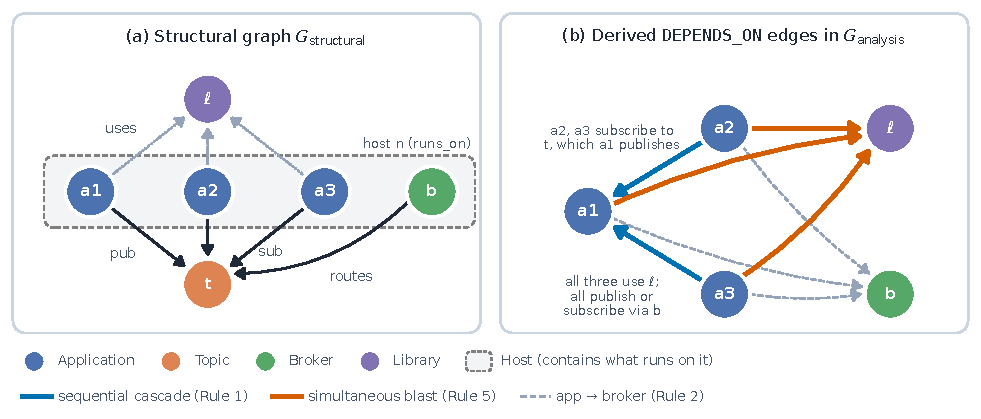
\includegraphics[width=\linewidth]{figures/Figure_2}
\caption{Running example: the raw structural graph (left) and the \texttt{DEPENDS\_ON} projection derived from it (right). The projection makes implicit runtime dependencies explicit---a subscriber depends on the publishers of its topics even though no structural edge joins them---while the simulators continue to operate on the structural view alone.}
\label{fig:supp-running}
\end{figure}

\section{Identification Quality Beyond Top-$K$ Overlap}
\label{supp:identification}

Every Overlap@$K$ figure in the main manuscript is a set-overlap measure: the
predicted and reference sets both contain exactly $K = \operatorname{round}(0.20
\cdot |V_{\text{app}}|)$ members, so precision, recall and $F_1$ take the same
value by construction. That quantity is well defined and we report it as
overlap, but it cannot distinguish a predictor that finds the critical set from
one that merely produces a set of the right size. Table~\ref{tab:identification}
reports three quantities that can, at operating points where precision and
recall are free to differ.

The LOSO block reproduces the paper's central negative finding on a different
family of metrics: \texttt{HGT-QoS} ($F_1@\tau = 0.383$, PR-AUC $0.471$),
\texttt{GAT-N-QoS} ($0.384$, $0.460$) and \texttt{Topo-QoS} ($0.358$, $0.469$)
are indistinguishable, and \texttt{HGT} attains the best PR-AUC of the seven
($0.477$). Identification therefore separates the predictors no better than
ranking does. The real-world block is where the two harnesses disagree: there
the learned model leads on both measures by a wide margin ($0.473$ and $0.713$
against $0.29$--$0.33$ and $0.47$--$0.52$), consistent with the full-population
transfer result of Table~12 of the main manuscript and subject to the same
caveat, that five systems cannot establish it.

\begin{table}[htbp]
\centering
\small
\centering
\caption{Identification quality at operating points where precision and recall are free to differ, so that none of these columns is the top-$K$ overlap measure reported as Overlap@$K$ elsewhere. $F_1@\tau$ scores the top-$K$ prediction against the labels' own critical set ($I^*(v) \ge 0.5\max I^*$); PR-AUC is threshold-free; nDCG@10 is rank-weighted. LOSO figures are means over the twelve inductive folds; real-world figures are means over the five transcribed systems, scored zero-shot against the same oracle.}
\label{tab:identification}
\begin{tabular}{lccc}
\toprule
Predictor & $F_1@\tau$ & PR-AUC & nDCG@10 \\
\midrule
\multicolumn{4}{l}{\textit{Inductive LOSO, twelve folds}} \\
\textsc{Topo} & 0.336 & 0.442 & 0.522 \\
\textsc{Topo-QoS} & 0.358 & 0.469 & 0.524 \\
\textsc{RM} & 0.302 & 0.403 & 0.469 \\
\textsc{GAT-N} & 0.294 & 0.388 & 0.409 \\
\textsc{GAT-N-QoS} & 0.384 & 0.460 & 0.498 \\
\textsc{HGT} & 0.372 & 0.477 & 0.553 \\
\textbf{HGT-QoS} & 0.383 & 0.471 & 0.501 \\
\midrule
\multicolumn{4}{l}{\textit{Zero-shot transfer, five open-source systems}} \\
RM & 0.287 & 0.521 & — \\
Topo & 0.329 & 0.474 & — \\
Topo-QoS & 0.329 & 0.474 & — \\
HGT-QoS & 0.473 & 0.713 & — \\
\bottomrule
\end{tabular}
\end{table}

\noindent\emph{Rendered by} \path{reproduce/render_table.py} \emph{from} \path{results/loso_all_variants_v5.json} \emph{and} \path{results/realworld_zeroshot_v7.json}.

\section{The $2\times2$ on a Variance-Stabilised Scale}
\label{supp:fisherz}

\noindent\textbf{Scope note.} This section analyses the \emph{unmatched} $2\times2$ of Table~10 of the main manuscript. The capacity- and channel-matched control (Table~11 of the main manuscript) removes the interaction and the typing effect entirely, so these robustness checks establish only that the unmatched interaction is not a metric or seed artefact, not that it reflects typing.

Spearman $\rho$ is bounded on $[-1, 1]$ and compresses toward either end. A
difference of differences computed on it is therefore not scale-free: two
mechanisms that each move a predictor toward the attainable ceiling can appear
sub-additive even if they contribute independently under any monotone
rescaling. Since the sub-additivity claim of Section~7.2 of the main manuscript
\emph{is} a claim about an interaction, it has to survive the transformation
that removes that artefact.

Table~\ref{tab:contrasts_z} repeats the three orthogonal quantities of the
$2\times2$ with each fold's $\rho$ passed through $\operatorname{arctanh}$
before the contrasts are formed. No cell of the shipped artifact reaches
$|\rho| = 1$, so the transform is finite throughout. The interaction does not
weaken; it grows, from $-0.199$ to $-0.233$, remains negative on all twelve
folds, and its bootstrap interval continues to exclude zero. Both main effects
likewise survive. Sub-additivity on this corpus is therefore a property of the
two mechanisms and not of the metric, which is what licenses reading typing and
the QoS edge channel as substitutes --- subject, as in the main text, to the
capacity and directionality confounds that the unrun control arms would
separate.

\begin{table}[htbp]
\centering
\small
\caption{The three orthogonal quantities of the $2\times2$ on the raw Spearman
scale and on the Fisher $z$ scale, Holm-corrected within each block of three.
Main effects average over the other factor's levels. \textbf{Won} counts folds
with $\Delta > 0$; the interaction is negative on all twelve under both
transformations. Post-hoc and exploratory, as in the main text.}
\label{tab:contrasts_z}
\begin{tabular}{lrrrr}
\toprule
\textbf{Quantity} & \textbf{$\Delta$ (raw $\rho$)} & \textbf{$\Delta$ (Fisher $z$)} & \textbf{Won} & \textbf{$p_{\text{Holm}}$} \\
\midrule
Typing (main effect)          & $+0.134$ & $+0.186$ & 12/12 & 0.0015 \\
QoS channel (main effect)     & $+0.187$ & $+0.269$ & 11/12 & 0.0015 \\
Typing $\times$ QoS interaction & $-0.199$ & $-0.233$ & 0/12 & 0.0015 \\
\midrule
\multicolumn{5}{l}{\textit{Interaction bootstrap 95\% CI: $[-0.258, -0.147]$ raw; $[-0.309, -0.165]$ on $z$}} \\
\bottomrule
\end{tabular}
\end{table}

\section{In-Distribution Per-Scenario Results}
\label{supp:indist-table}

This table was moved out of the body because no comparison can be drawn down its columns: the typed and homogeneous arms read different substrates in-distribution (Section~6.2.1 of the main manuscript), so a difference between them confounds message passing with multi-entity visibility. It is retained because the per-scenario cells expose within-predictor fitting behaviour that the fold means hide.

\begin{table}[htbp]
\centering
\small
\caption{In-distribution held-out evaluation across all twelve distributed architecture scenarios, reporting both Spearman rank correlation ($\rho$) and critical-set identification (Overlap@$K$, with $K = \text{round}(0.20 \cdot n)$): mean over five seeds; $n$ = held-out Application test count. Overlap@$K$ is top-$K$ set overlap throughout (Section 6.3 of the main manuscript). Substrates differ in-distribution and are listed per predictor in Table 6 (Section 6.2 of the main manuscript). Each seed redraws the 60/20/20 split and model initialization. The held-out set is small on several scenarios --- $n = 5$ on ATM, giving $K = 1$ --- so a single rank swap moves $\rho$ substantially and the per-scenario cells on the smaller topologies are coarsely quantized; they are reported for completeness and the row means, not individual cells, carry the comparison.}
\label{tab:supp-indist-cells}
\resizebox{\linewidth}{!}{%
\begin{tabular}{lrcccccccccccc}
\toprule
\textbf{Scenario} & \textbf{$n$} & \multicolumn{2}{c}{\textbf{Topo}} & \multicolumn{2}{c}{\textbf{Topo-QoS}} & \multicolumn{2}{c}{\textbf{GAT}} & \multicolumn{2}{c}{\textbf{GAT-QoS}} & \multicolumn{2}{c}{\textbf{HGT}} & \multicolumn{2}{c}{\textbf{HGT-QoS}} \\
\cmidrule(lr){3-4} \cmidrule(lr){5-6} \cmidrule(lr){7-8} \cmidrule(lr){9-10} \cmidrule(lr){11-12} \cmidrule(lr){13-14}
& & $\rho$ & $F_1$ & $\rho$ & $F_1$ & $\rho$ & $F_1$ & $\rho$ & $F_1$ & $\rho$ & $F_1$ & $\rho$ & $F_1$ \\
\midrule
\textbf{ATM System} & 5 & 0.538 & 0.400 & 0.557 & 0.400 & $-$0.393 & 0.000 & $-$0.080 & 0.000 & 0.492 & 0.600 & 0.348 & 0.400 \\
\textbf{AV System} & 16 & 0.188 & 0.333 & 0.797 & 0.533 & 0.816 & 0.400 & 0.465 & 0.267 & 0.637 & 0.533 & 0.558 & 0.533 \\
\textbf{Enterprise} & 60 & 0.443 & 0.600 & 0.793 & 0.600 & 0.779 & 0.583 & 0.481 & 0.433 & 0.861 & 0.600 & 0.878 & 0.600 \\
\textbf{Financial Trading} & 12 & 0.387 & 0.200 & 0.512 & 0.400 & 0.565 & 0.400 & 0.666 & 0.400 & 0.693 & 0.500 & 0.730 & 0.500 \\
\textbf{Healthcare} & 10 & 0.291 & 0.200 & 0.399 & 0.000 & 0.725 & 0.300 & 0.575 & 0.300 & 0.575 & 0.400 & 0.607 & 0.500 \\
\textbf{Enterprise Integration (ESB)} & 14 & 0.179 & 0.267 & 0.429 & 0.400 & 0.363 & 0.467 & $-$0.156 & 0.067 & 0.421 & 0.400 & 0.476 & 0.400 \\
\textbf{Industrial SCADA} & 28 & 0.601 & 0.533 & 0.710 & 0.533 & 0.656 & 0.533 & 0.478 & 0.500 & 0.787 & 0.667 & 0.839 & 0.633 \\
\textbf{IoT Smart City} & 40 & 0.320 & 0.350 & 0.397 & 0.350 & 0.580 & 0.450 & 0.538 & 0.425 & 0.849 & 0.650 & 0.850 & 0.650 \\
\textbf{Logistics Fleet} & 22 & 0.511 & 0.500 & 0.652 & 0.400 & 0.746 & 0.500 & 0.780 & 0.550 & 0.796 & 0.550 & 0.815 & 0.500 \\
\textbf{Microservices (synthetic)} & 18 & 0.219 & 0.150 & 0.344 & 0.250 & 0.351 & 0.400 & 0.363 & 0.450 & 0.141 & 0.300 & 0.664 & 0.600 \\
\textbf{Real-Time Gaming} & 15 & 0.360 & 0.533 & 0.802 & 0.533 & 0.464 & 0.333 & 0.471 & 0.400 & 0.651 & 0.533 & 0.641 & 0.400 \\
\textbf{Telecom RAN} & 24 & 0.402 & 0.480 & 0.422 & 0.280 & 0.608 & 0.320 & 0.350 & 0.360 & 0.591 & 0.280 & 0.526 & 0.320 \\
\midrule
\textbf{Mean} & — & 0.370 & 0.379 & 0.568 & 0.390 & 0.522 & 0.391 & 0.411 & 0.346 & 0.624 & 0.501 & 0.661 & 0.503 \\
\bottomrule
\end{tabular}%
}
\end{table}

\section{Results at a Glance}
\label{supp:glance}

The panels below restate Tables~8, 9 and 10 of the main manuscript graphically, together with the inter-oracle agreement of Section~7.3.2. Nothing here is a new measurement; the figure is retained for readers who prefer the visual summary.

\begin{figure}[htbp]
\centering
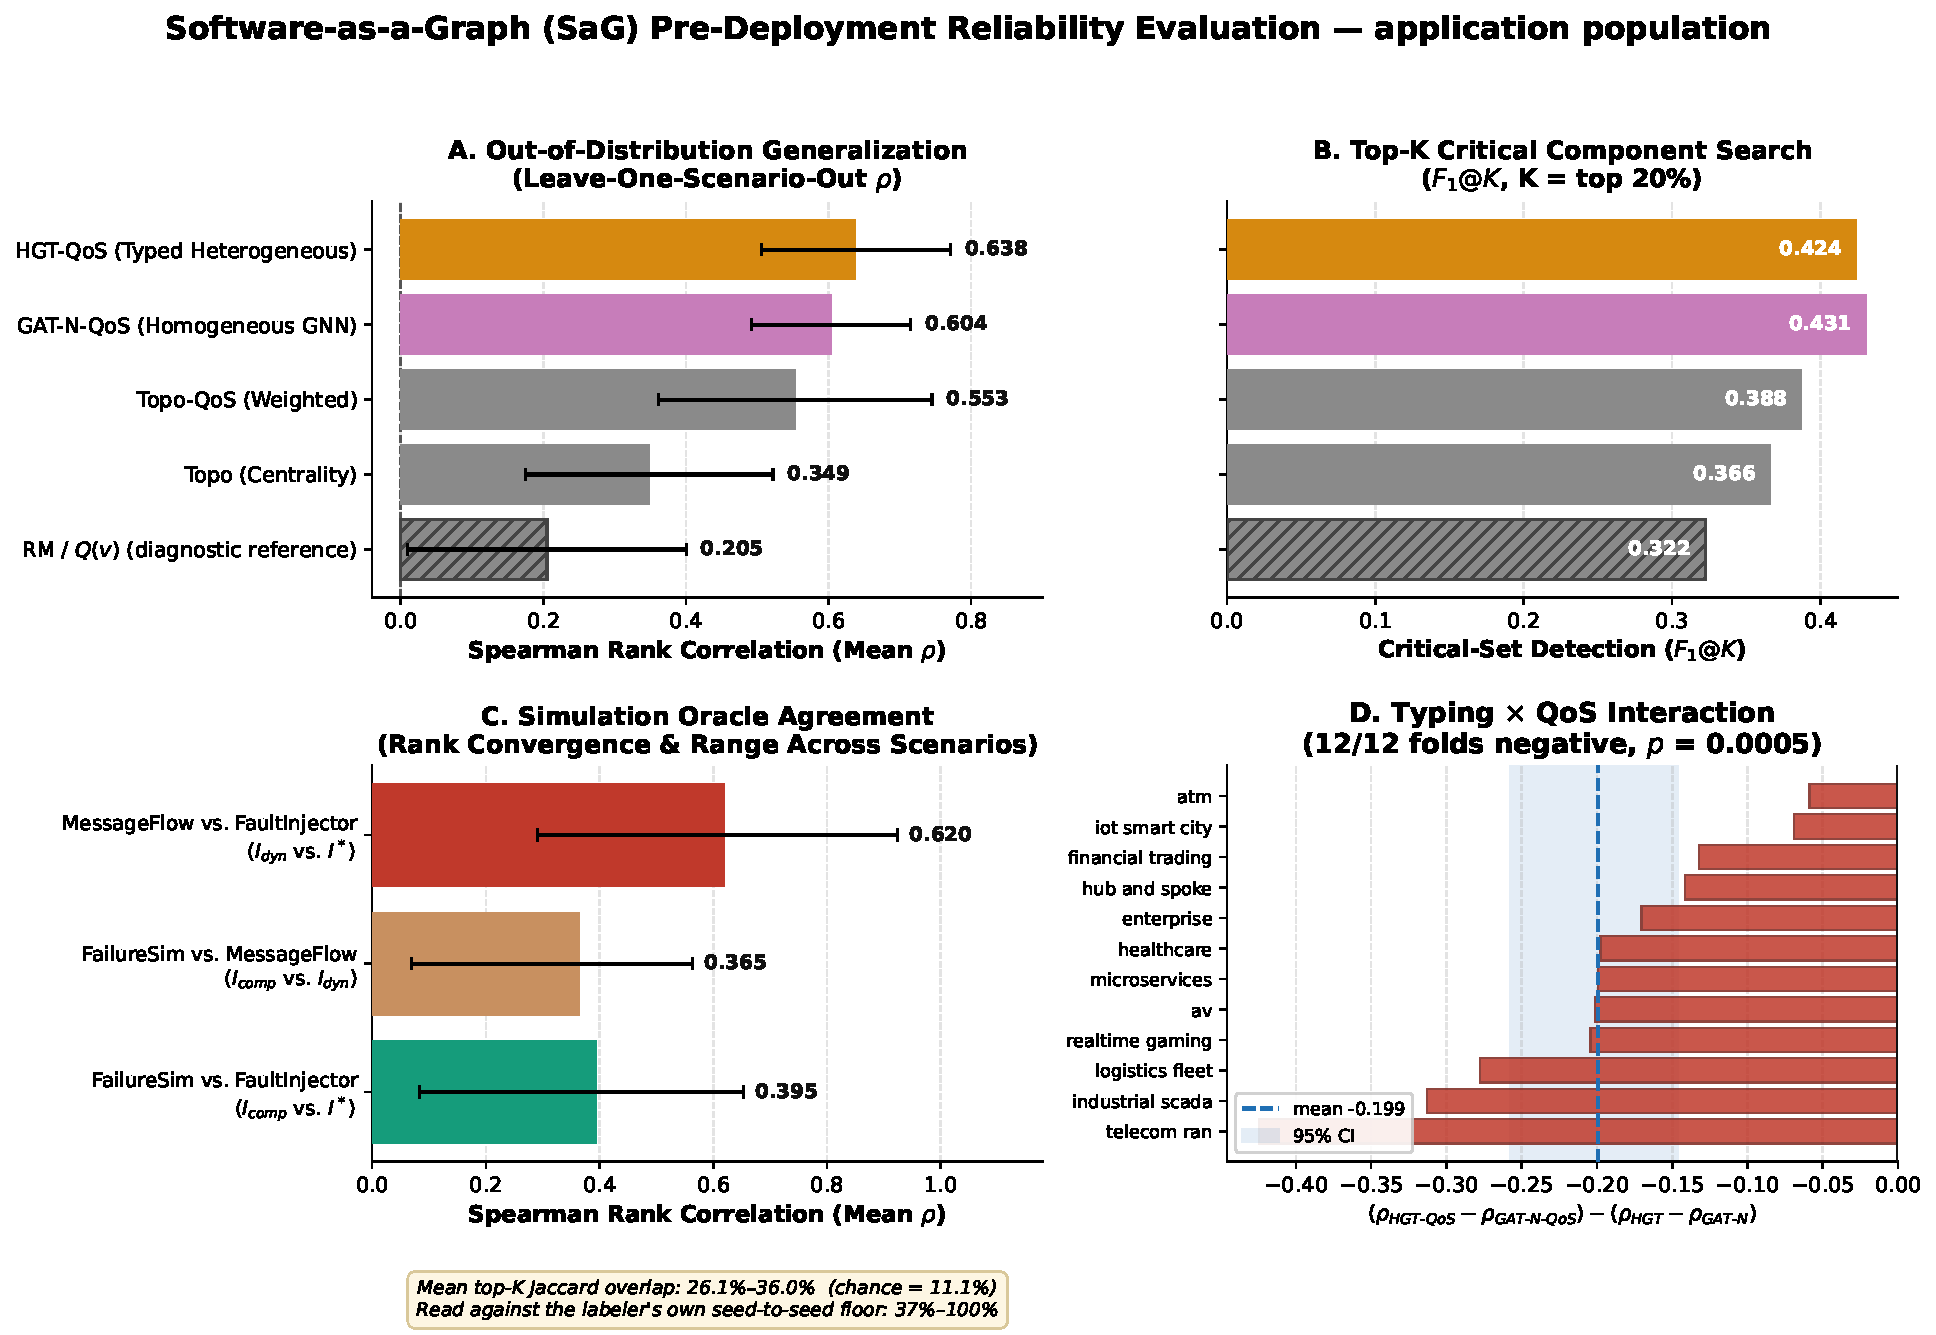
\includegraphics[width=0.72\linewidth]{figures/Figure_3}
\caption{Results at a glance: Application population. \textbf{(A)} Out-of-distribution rank correlation per predictor across the twelve LOSO folds. \textbf{(B)} Critical-set identification at $K = 20\%$, where the typed model does not separate from untyped learning. \textbf{(C)} Pairwise rank agreement between the three simulation oracles, against the chance baseline. \textbf{(D)} The typing $\times$ QoS interaction per fold, negative on all twelve (Section 7.2 of the main manuscript); the dashed line is the mean and the band its bootstrap 95\% CI. Panels A and B are read from the same artifact as Table 8 of the main manuscript, C from the convergent-validity artifact, and D from the significance artifact behind Table 10 of the main manuscript.}
\label{fig:supp-glance}
\end{figure}

\section{Illustrative Diagnostic Remediation Card}
\label{supp:card}

The card below is composed by hand from the ATM topology to show the shape of the explanation layer's output. It is an illustration of the format, not a measured export, and no claim rests on it.

\begin{table}[htbp]
\centering
\small
\caption{Illustrative Diagnostic Remediation Card for a flagged component (\texttt{TransactionProcessor} in the ATM System case study). The explanation layer maps structural metrics to ISO/IEC sub-characteristics to guide engineering intervention.}
\label{tab:supp-card}
\resizebox{\linewidth}{!}{%
\begin{tabular}{lll}
\toprule
\textbf{Diagnostic Attribute} & \textbf{Evaluated Value} & \textbf{Structural Interpretation} \\
\midrule
\textbf{Component ID} & \texttt{TransactionProcessor} & Core transaction coordinator ($V_{\text{app}}$) \\
\textbf{Tukey Risk Tier} & \textbf{CRITICAL} & $Q(v) = 0.84 > Q_3 + 1.5 \cdot \text{IQR}$ \\
\midrule
\multicolumn{3}{l}{\textit{ISO/IEC 25010 Structural Quality Profile Breakdown}} \\
\textbf{Availability ($A$)} & $0.89$ [High SPOF Risk] & $\text{AP}_c^{\text{dir}} = 1.00$, $\text{QSPOF} = 0.92$, $\text{CDI} = 0.78$ \\
\textbf{Fault Tolerance ($FT$)} & $0.31$ [Low Cascade Propagation] & $\text{RPR} = 0.25$, $\text{Deg}_{\text{in}} = 0.30$, $\text{CDPot} = 0.38$ \\
\textbf{Maintainability ($M$)} & $0.65$ [Moderate Structural Coupling] & $\text{BT} = 0.70$, $w_{\text{out}} = 0.60$, $\text{CQP} = 0.40$ \\
\midrule
\textbf{Structural Diagnosis} & \multicolumn{2}{l}{Isolated Single Point of Failure (Severe $A$ deficit, low downstream cascade reach)} \\
\textbf{Prescriptive Action} & \multicolumn{2}{l}{Deploy warm-standby replica and establish redundant message broker routing} \\
\bottomrule
\end{tabular}%
}
\end{table}


\section{General Multi-Task Objective}
\label{supp:objective}

The implementation supports a more general objective than the one optimized in every reported run (Eq.~5 of the main manuscript):
\begin{equation}
\mathcal{L} = \mathcal{L}_{\text{composite}} + 0.5 \cdot \mathcal{L}_{\text{dimension}} + 0.3 \cdot \mathcal{L}_{\text{rank}} + 0.1 \cdot \mathcal{L}_{\text{pairwise}} + \lambda_{\text{RM}} \cdot \mathcal{L}_{\text{consistency}},
\end{equation}
where $\mathcal{L}_{\text{dimension}} = \frac{1}{\sum_{d} m_d} \sum_{d \in \{R, M\}} m_d \cdot \text{MSE}(\hat{d}(v), d^*(v))$ uses a boolean dimension mask $m = [m_R, m_M]$, and $\mathcal{L}_{\text{consistency}}$ is an optional mean-squared alignment of the two auxiliary heads with the explanation layer's $R$ and $M$ scores on unlabeled nodes. Every reported run sets $\lambda_{\text{RM}} = 0$, so the predictor and the explanation layer share no parameters, and $m = [1, 0]$ with $R^*(v) \equiv I^*(v)$, because no simulated maintainability label exists. Under these settings $\mathcal{L}$ reduces exactly to the active objective. The code also provides a domain reweighting $\hat{Q}_{\text{domain}}(v) = q_R \hat{a}_1(v) + q_M M_{\text{static}}(v)$ for an ISO/IEC 25019 context-of-use vector; it is not evaluated in this study.

\section{Seed-Aggregation Robustness of the \texorpdfstring{$2\times2$}{2x2}}
\label{supp:seed-robust}

\noindent\textbf{Scope note.} This section analyses the \emph{unmatched} $2\times2$ of Table~10 of the main manuscript. The capacity- and channel-matched control (Table~11 of the main manuscript) removes the interaction and the typing effect entirely, so these robustness checks establish only that the unmatched interaction is not a metric or seed artefact, not that it reflects typing.

\texttt{GAT-N}, the floor cell of the reported $2\times2$, has a median within-fold seed standard deviation of $0.298$, against $0.114$ (\texttt{HGT}), $0.024$ (\texttt{GAT-N-QoS}) and $0.052$ (\texttt{HGT-QoS}). If a few collapsed seeds pull its fold means down, both main effects and the interaction inherit that optimization failure. Table~\ref{tab:supp-seed-robust} re-forms each fold score from the per-seed results of the same twelve-fold artifact under three aggregations and recomputes the three orthogonal quantities, Holm-corrected across the three within each aggregation. No model is retrained (\path{reproduce/factorial_seed_robustness.py}; \path{results/factorial_seed_robustness_v5.json}).

\begin{table}[htbp]
\centering
\small
\caption{The $2\times2$ quantities of Table~10 (main manuscript) under three seed aggregations. \emph{Mean} reproduces the reported table; \emph{median} is robust to one or two collapsed seeds per fold; \emph{trimmed} drops each arm's worst seed in every fold before averaging. CI: bootstrap over folds ($B = 2{,}000$).}
\label{tab:supp-seed-robust}
\begin{tabular}{llrcccc}
\toprule
\textbf{Aggregation} & \textbf{Quantity} & \textbf{$\Delta\rho$} & \textbf{Won} & \textbf{$p$} & \textbf{$p_{\text{Holm}}$} & \textbf{95\% CI} \\
\midrule
Mean & Typing (main) & $+0.134$ & 12/12 & 0.0005 & 0.0015 & $[+0.095, +0.176]$ \\
 & QoS channel (main) & $+0.187$ & 11/12 & 0.0015 & 0.0015 & $[+0.108, +0.244]$ \\
 & Interaction & $-0.199$ & 0/12 & 0.0005 & 0.0015 & $[-0.258, -0.147]$ \\
\midrule
Median & Typing (main) & $+0.118$ & 11/12 & 0.0010 & 0.0020 & $[+0.067, +0.175]$ \\
 & QoS channel (main) & $+0.145$ & 11/12 & 0.0093 & 0.0093 & $[+0.070, +0.206]$ \\
 & Interaction & $-0.168$ & 0/12 & 0.0005 & 0.0015 & $[-0.231, -0.112]$ \\
\midrule
Trimmed & Typing (main) & $+0.118$ & 11/12 & 0.0010 & 0.0020 & $[+0.077, +0.160]$ \\
 & QoS channel (main) & $+0.128$ & 11/12 & 0.0093 & 0.0093 & $[+0.060, +0.179]$ \\
 & Interaction & $-0.146$ & 0/12 & 0.0005 & 0.0015 & $[-0.177, -0.115]$ \\
\bottomrule
\end{tabular}
\end{table}

\noindent The interaction shrinks by a sixth (median) to a quarter (trimmed) and stays negative on every fold, and the QoS-channel main effect shrinks most. Collapsed \texttt{GAT-N} seeds therefore inflate the reported effects but do not produce them. The check cannot address under-training that affects every seed alike, which requires per-arm tuning under an equal budget.


\section{Closed-Form Scores With the Articulation Term Restored}
\label{supp:ap-sensitivity}

The closed-form scores are specified as $0.6\cdot\text{BT} + 0.4\cdot\text{AP}$ (Section~6.2.1 of the main manuscript). In the evaluated implementation the articulation term reads zero for every node, because the cached structural metrics carry no articulation score. Table~\ref{tab:supp-ap} recomputes both scores on the same twelve holdouts, Application population and $I^*(v)$ labels, with the articulation term taken from the articulation severity SaG computes on the projection (\path{reproduce/topo_ap_sensitivity.py}; \path{results/topo_ap_sensitivity.json}). The \emph{as run} columns reproduce the published per-fold values exactly (maximum absolute difference $<10^{-15}$).

\begin{table}[htbp]
\centering
\small
\caption{Spearman $\rho$ of the closed-form scores per LOSO holdout, as run (articulation term zero) and with the articulation term restored. $n_{\text{AP}}$ counts nodes with non-zero articulation severity on the projection.}
\label{tab:supp-ap}
\begin{tabular}{lrcccc}
\toprule
\textbf{Holdout} & $n_{\text{AP}}$ & \textbf{Topo, as run} & \textbf{Topo, AP restored} & \textbf{Topo-QoS, as run} & \textbf{Topo-QoS, AP restored} \\
\midrule
ATM & 1 & 0.256 & 0.083 & 0.311 & 0.132 \\
AV System & 0 & 0.468 & 0.468 & 0.753 & 0.753 \\
Enterprise & 0 & 0.431 & 0.431 & 0.795 & 0.795 \\
Financial Trading & 0 & 0.237 & 0.237 & 0.586 & 0.586 \\
Healthcare & 0 & 0.077 & 0.077 & 0.369 & 0.369 \\
Enterprise Integration (ESB) & 0 & 0.112 & 0.112 & 0.430 & 0.430 \\
Industrial SCADA & 10 & 0.608 & 0.563 & 0.650 & 0.609 \\
IoT Smart City & 6 & 0.251 & 0.234 & 0.351 & 0.331 \\
Logistics Fleet & 2 & 0.576 & 0.578 & 0.741 & 0.742 \\
Microservices & 0 & 0.229 & 0.229 & 0.265 & 0.265 \\
Real-Time Gaming & 0 & 0.377 & 0.377 & 0.810 & 0.810 \\
Telecom RAN & 0 & 0.562 & 0.562 & 0.576 & 0.576 \\
\midrule
\textbf{Mean} & & \textbf{0.349} & \textbf{0.329} & \textbf{0.553} & \textbf{0.533} \\
\bottomrule
\end{tabular}
\end{table}

\noindent Articulation points are rare on these projections (four of twelve scenarios have any), and where they exist the binary term lowers the ranking correlation. The evaluated, betweenness-only form is therefore the stronger reference, and every comparison in the main manuscript is made against it.


\section{SaG-Hybrid Per-Fold Results}
\label{supp:hybrid-folds}

Table~\ref{tab:supp-hybrid} lists the per-fold Spearman $\rho$ behind Table~14 of the main manuscript: one CPU sweep, twelve LOSO folds, fold score = mean over five seeds, Application population (\path{results/loso_hybrid_cpu.json}). Folds are ordered by the closed-form engine's own score. SaG-Hybrid outperforms \texttt{Topo-QoS} on every fold except Enterprise, and keeps most of the closed-form engine's strength on the folds where \texttt{HGT-QoS} loses to it.

\begin{table}[htbp]
\centering
\small
\caption{Per-fold LOSO $\rho$ for SaG's closed-form, learned and hybrid engines (CPU sweep; bold marks the best of the three).}
\label{tab:supp-hybrid}
\begin{tabular}{lcccc}
\toprule
\textbf{Holdout} & \textbf{Topo-QoS} & \textbf{HGT-QoS} & \textbf{SaG-Hybrid} & \textbf{Hybrid $-$ Topo-QoS} \\
\midrule
Real-Time Gaming & 0.810 & 0.789 & \textbf{0.837} & $+0.026$ \\
Enterprise & \textbf{0.795} & 0.426 & 0.734 & $-0.061$ \\
AV System & 0.753 & 0.704 & \textbf{0.782} & $+0.029$ \\
Logistics Fleet & 0.741 & 0.771 & \textbf{0.792} & $+0.051$ \\
Industrial SCADA & 0.650 & 0.684 & \textbf{0.758} & $+0.108$ \\
Financial Trading & 0.586 & 0.695 & \textbf{0.754} & $+0.167$ \\
Telecom RAN & 0.576 & 0.427 & \textbf{0.648} & $+0.071$ \\
Enterprise Integration (ESB) & 0.430 & 0.548 & \textbf{0.564} & $+0.135$ \\
Healthcare & 0.369 & \textbf{0.730} & 0.625 & $+0.256$ \\
IoT Smart City & 0.351 & \textbf{0.688} & 0.590 & $+0.239$ \\
ATM & 0.311 & \textbf{0.523} & 0.429 & $+0.118$ \\
Microservices & 0.265 & \textbf{0.475} & 0.366 & $+0.100$ \\
\midrule
\textbf{Mean} & 0.553 & 0.622 & \textbf{0.657} & $+0.103$ \\
\bottomrule
\end{tabular}
\end{table}

\end{document}
